\documentclass{amsart}
\linespread{2}
\input{assets/preamble.tex}

\begin{document}
\author{Daniel Cicala}
\title{Rewriting structured cospans}
\date{\today}
\email{dcicala@newhaven.edu}
\address{Department of Mathematics and Physics\\
  University of New Haven}
\maketitle

\begin{abstract}
  To foster the study of networks on an abstract level, we
  further study the formalism of \emph{structured cospans}
  introduced by Baez and Courser. A structured cospan is a
  diagram of the form $ La \to x \gets Lb $ built from a
  geometric morphism with left exact left adjoint
  $ L \dashv R \from \X \to \A $.  We show that this
  construction is functorial and results in a topos with
  structured cospans for objects.  Additionally, structured
  cospans themselves are compositional. Combining these two
  perspectives, we define a double category of structured
  cospans.  We then leverage adhesive categories to create a
  theory of rewriting for structured cospans. We generalize
  the result from graph rewriting stating that a graph
  grammar induces the same rewrite relation as its
  underlying graph grammar.  We use this fact to prove our
  main result, a complete characterization of the rewriting
  relation for a topos $ \X $ using double categories.  This
  provides a compositional framework for rewriting systems.
\end{abstract}


%% ===================================
%% Introduction
%% ===================================
\section{Introduction}
\label{sec:Intro}


%% ===================================
%% Rewriting in Topoi
%% ===================================
\section{Rewriting in topoi}
\label{sec:RewriteTopoi}

The topic of double pushout rewriting is well represented in
the literature. Here, we cover the basics and set our
notation and convention. Experts can skip to the next
section. Novices have many suitable choices to supplement
this review, though we suggest Lack and Sobocinski's
axiomatization of rewriting in adhesive categories
\cite{LackSobo_Adhesive}.

Rewriting starts with the notion of a \df{rewrite rule}, or
simply \df{rule}. In its most general form, a rule is a span
\[
  \ell \gets k \to r
\]
in a topos. For us, the arrows are of the span are always
monic and, whenever possible, unnamed.

The conceit of a rule is that $ r $ replaces $ \ell $ while
$ k $ identifies a subsystem of $ \ell $ that remains
fixed. For example, suppose we were modeling some system
using graphs where self-loops are negligable. For example,
consider a model of the internet as a graph with websites
for nodes and links for edges. If we wished to ignore links
from a websites to itself, we can introduce a rule
that replaces a loop on a node with that node
\begin{equation}\label{eq:squashLoopRule}
  \begin{tikzpicture}[
    baseline=(current bounding box.center),
    scale=0.75]
    \draw [rounded corners]
      (-1,-1) rectangle (1,2);
    \node (a)  at (0,0.5)   {$ \bullet $};
    \node (lr) at (1.1,0.5) {};  
    \draw [graph,loop above] (a) to (a);
    %
    \draw [rounded corners]
      (2,-1) rectangle (4,2);
    \node (b)  at (3,0.5)   {$ \bullet $};
    \node (ml) at (1.9,0.5) {};
    \node (mr) at (4.1,0.5) {};
    %
    \draw [rounded corners]
      (5,-1) rectangle (7,2);
    \node (c)  at (6,0.5) {$ \bullet $};
    \node (rl) at (4.9,0.5) {};
    %
    \draw [cd]
      (ml) edge node[]{$  $} (lr)
      (mr) edge node[]{$  $} (rl); 
 \end{tikzpicture}
 \end{equation}   

To \emph{apply} a rule $ \ell \gets k \to r $ to an object
$ \ell' $, we require an arrow $ \ell \to \ell' $ such that
there exists a \df{pushout complement}, an object $ d $
fitting into a pushout diagram \[
  \begin{tikzpicture}
    \node (l) at (0,2) {$ \ell $};
    \node (k) at (2,2) {$ k $};
    \node (g) at (0,0) {$ g $};
    \node (d) at (2,0) {$ d $};
    \draw [cd]
       (k) edge node[]{$  $}      (l)
       (k) edge node[]{$  $}      (d)
       (l) edge node[left]{$ m $} (g)
       (d) edge node[]{$  $}      (g); 
    \draw (0.3,0.4) -- (0.4,0.4) -- (0.4,0.3);
  \end{tikzpicture}
\] 
A pushout complement need not exist, but when it does and
the map $ k \to \ell $ is monic, then it is unique up to
isomorphism \cite[Lem.~15]{LackSobo_Adhesive}.

Each application of a rule begets a new rule.

\begin{definition}[Derived rule] \label{def:derived-rule}
  Applying a rule $ \ell \gets k \to r $ to an object $ g $
  induces a \df{derived rule} $ \ell' \gets k' \to r' $ that
  fits into the bottom row of the double pushout diagram
  \input{assets/derivedRule.tex}
\end{definition}

The arrows of derived rule are also monic because pushouts
in topoi preserve monics
\cite[Lem.~12]{lack-sobo_adhesive-cats}. Interpret this
diagram as follows: the map $ \ell \to \ell' $ selects a
copy of $ \ell $ inside $ \ell' $ and that copy is replaced
by $ r $ resulting in the new object $ r' $. 

To illustrate, let us return to the internet modeled using
graphs and negligable self-loops.  Then we can
apply Rule \eqref{eq:squash-loop-rule} to any node with a
loop. This application is captured with the double pushout
diagram \begin{equation} \label{eq:example-dpo-diagram}
 \begin{tikzpicture}
    \begin{scope} 
      \node (c) at (0,0.5) {$ \bullet $};
      \draw [graph,loop above]
        (c) edge (c);
      \draw [rounded corners]
        (-1,-1) rectangle (1,2);
      \node (01r) at (1.1,0)  {};
      \node (01b) at (0,-1.1) {};  
    \end{scope}
    %
    \begin{scope}[shift={(4,0)}]
      \node (c) at (0,0.5) {$ \bullet $};
      \draw [rounded corners]
        (-1,-1) rectangle (1,2);
      \node (11l) at (-1.1,0) {};
      \node (11r) at (1.1,0)  {};
      \node (11b) at (0,-1.1) {};
    \end{scope}
    %
    \begin{scope}[shift={(8,0)}]
      \node (c) at (0,0.5) {$ \bullet $};
      %
      \draw [rounded corners]
        (-1,-1) rectangle (1,2);
      \node (21l) at (-1.1,0) {};
      \node (21b) at (0,-1.1) {};
    \end{scope}
    %
    \begin{scope}[shift={(0,-5)}]
      \node (a) at (-0.5,-0.5) {$ \bullet $};
      \node (b) at (0.5,-0.5)  {$ \bullet $};
      \node (c) at (0,0.5)     {$ \bullet $};
      \draw [graph]
      (a) edge              (c)
      (b) edge              (c)
      (c) edge [loop above] (c);
      %
      \draw [rounded corners]
        (-1,-1) rectangle (1,2);
      \node (00t) at (0,2.1)   {};
      \node (00r) at (1.1,0.5) {};  
    \end{scope}
    %
    \begin{scope}[shift={(4,-5)}]
      \node (a) at (-0.5,-0.5) {$ \bullet $};
      \node (b) at (0.5,-0.5) {$ \bullet $};
      \node (c) at (0,1) {$ \bullet $};
      \draw [graph]
        (a) edge (c)
        (b) edge (c);
      %
      \draw [rounded corners]
        (-1,-1) rectangle (1,2);
      \node (10t) at (0,2.1)    {};
      \node (10r) at (1.1,0.5)  {};
      \node (10l) at (-1.1,0.5) {};
    \end{scope}
    %
    \begin{scope}[shift={(8,-5)}]
      \node (a) at (-0.5,-0.5) {$ \bullet $};
      \node (b) at (0.5,-0.5)  {$ \bullet $};
      \node (c) at (0,1)    {$ \bullet $};
      \draw [graph]
      (a) edge              (c)
      (b) edge              (c);
      %
      \draw [rounded corners]
        (-1,-1) rectangle (1,2);
      \node (20t) at (0,2.1)    {};
      \node (20l) at (-1.1,0.5) {};
      \end{scope}
      % 
      \draw [cd]
      (01b) edge node[left]{$ m $} (00t)
      (11b) edge (10t)
      (21b) edge (20t)
      (11l) edge (01r)
      (11r) edge (21l)
      (10l) edge (00r)
      (10r) edge (20l);
    \end{tikzpicture}
  \end{equation}

  


The map $ m $ selects the self-loop and corresponding node
in the bottom left graph. A pushout complement exists,
meaning that the rule can be applied and so the loop is
removed. The result is the bottom right graph.  The reader
can check that the two squares are pushouts.

Specialists is a particular sort of system spend time
understanding the its rewrite rules. Resistor circuits have
parallel, series, and star rules. Other systems have their
own versions. Therefore, we consider a system equipped with
a set of rules. 

\begin{definition}[Grammar] \label{def:grammar} A topos
  $ \T $ together with a finite set $ P $ of rules
  $ \{ \spn{\ell_j}{k_j}{r_j} \} $ in $ \T $ is a
  \df{grammar}. A morphisms of grammars
  $ ( \cat{S} , P ) \to ( \T , Q ) $ is a pullback and pushout
  preserving functor $ F \from \cat{S} \to \T $ such that for
  each rule $ \xspn{\ell}{f}{k}{g}{r} $ in $ P $, the rule
  $ \xspn{F\ell}{Ff}{Fk}{Fg}{Fr} $ is in $ Q $. Together
  these form a category $ \Gram $.
\end{definition}

Like a seed, from a grammar grows something entirely new
called the \emph{language}. The language contains all necessary
information about the syntax of a system, so naturally, it
is the thing to study. The potential complexity of a
language makes this a difficult task, so we instead turn to
a more accessible proxy called the \emph{rewrite
  relation}. This relation captures the relationship between
the many sytactical componenets of a language.  

Constructing the rewrite relation requires several steps.  A
grammar $ ( \T , P ) $ induces a relation
$ \dderiv{}{} $ on the objects of $ \T $ defined by
$ \dderiv{g}{h} $ whenever there exists a rule
$ \spn{g}{d}{h} $ derived from a production in $ P $. For
instance, the above double pushout diagram would relate
\[
  \begin{tikzpicture}
    \begin{scope}[shift={(0,0)}]
      \node (a) at (-0.5,-0.5) {$ \bullet_a $};
      \node (b) at (0.5,-0.5)  {$ \bullet_b $};
      \node (c) at (0,0.5)     {$ \bullet_c $};
      \draw [graph]
        (a) edge              (c)
        (b) edge              (c)
        (c) edge [loop above] (c); 
      %
      \draw [rounded corners]
        (-1,-1) rectangle (1,2);
    \end{scope}
    %
    \node at (1.5,0.5) {$ \dderiv{}{} $};
    %
    \begin{scope}[shift={(3,0)}]
      \node (a) at (-0.5,-0.5) {$ \bullet_a $};
      \node (b) at (0.5,-0.5)  {$ \bullet_b $};
      \node (c) at (0,0.5)       {$ \bullet_c $};
      \draw [graph]
        (a) edge              (c) 
        (b) edge              (c);
      \draw [rounded corners]
        (-1,-1) rectangle (1,2);
    \end{scope}
  \end{tikzpicture}
\]

But $ \dderiv{}{} $ is too small to capture the full
behavior of the language.  For one, it is not true in
general that $ \dderiv{g}{g} $ holds. Also, $ \dderiv{}{} $
does not capture multi-step rewrites. That is, there may be
derived rules witnessing $ \dderiv{g}{g'} $ and
$ \dderiv{g'}{g''} $ but not a derived rule witnessing
$ \dderiv{g}{g''} $. We want to relate a pair of objects if
one can be rewritten into another using a finite sequence of
rules that are either in $ P $ or derived from a rule in
$ P $. Therefore, we define the \df{rewrite relation} to be
the reflexive and transitive closure of $ \dderiv{}{} $

After we introduce a grammar for structured cospans in Section
\ref{sec:}, we show that constructing it is functorial.

%% ===========================================
\section{Structured cospans form a topos}
\label{sec:StructureOfStrCsp}
%% ===========================================

Having discussed rewriting in a topos, in order to introduce
the rewriting of structured cospans, we better ensure that
they form a topos. Indeed, we do this after recalling their
definition.

Baez and Courser introduced structured cospans
\cite{bc_strCsp} to serve as a syntax for open systems. We
use the term `system' broadly and avoid giving a precise
definition.  By `open', we mean that compatible systems can
be connected to form a larger system.  For example, a vacuum
cleaner can connected to the electrical grid via an
electrical socket. Or, a pulley system can connect to a
mechanical motor.

In order to form a topos out of structured cospans, we require stronger conditions than assumed by Baez and Courser.

%% define structured cospans
\begin{definition}
  Fix an adjunction $$\adjunction{\X}{L}{R}{\A}$$ between
  (elementary) topoi with $ L $ preserving finite
  limits. An \df{$ L $-structured
    cospan}, or simply \df{structured cospan}, is any cospan
  in $ \X $ of the form $ La \to x \gets Lb $.    
\end{definition}

How does the structured cospan syntax map onto an open
system? The apex $x$ of the cospan represents the system
itself.  The legs of the cospan, $ La \to x $ and
$ Lb \to x $, select the inputs $ La $ and outputs $ Lb $ of
$ x $. These legs endow structured cospans with the ability
to connect together. Given $ La \to x \gets Lb $ and
$ Lb \to y \gets Lc $, we form the \emph{composite}
structured cospan $ La \to x+_{Lb}y \gets Lc $. Interpret
the pushout $ x+_{Lb}y $ as an object obtained by glueing
$ x $ to $ y $ along their common interface $ Lb $. The
reason we call $La \gets x+_{Lb}y \to Lc$ the `composite' is
because a natural way to emphasize this connectability is by
defining a category in which structured cospans are the
arrows.

%% define category w str cospans as arrows
\begin{definition}
  Given an adjunction $$\adjunction{\X}{L}{R}{\A}$$ between
  (elementary) topoi with $ L $ preserving finite limits,
  denote by $ _L \Csp $ the category whose objects are those
  of $ \A $ and arrows from $ a $ to $ b $ are structured
  cospans $ La \to x \gets Lb $.  
\end{definition}

Of course, $ _L \Csp $ does not require the full strength of
those conditions to form a category---Baez and Courser do
not ask this much---but remember, we are aiming to form a
topos of structured cospans.

%% example: open graphs
\begin{example}
  Consider the
  adjunction $$\adjunction{\Graph}{L}{R}{\Set}$$ with $ L $
  the discrete graph functor and $ R $ the functor that
  forgets the graph edges.  Structured cospans for this
  adjunction are open graphs, that is graphs equipped with
  two subset of nodes, one set interpretted as inputs and
  the other as outputs. These ``interface'' sets need not be
  disjoint. For example, the pair of open graphs
  \begin{center}
\begin{tikzpicture}[scale=0.5]
  \begin{scope}
    \node (1) at (0,0) {{$ _a \bullet $}};
    \node (2) at (0,2) {{$ _b \bullet $}};
    \node (3) at (2,2) {{$ \bullet_d $}};
    \node (4) at (2,0) {{$ \bullet_e $}};
    \node (5) at (1,4) {{$ \bullet_c $}};
    %
    \draw [graph]
    (1) edge[] (2)
    (2) edge[] (3)
    (3) edge[] (1)
    (4) edge[] (3)
    (3) edge[] (5)
    (5) edge[] (2);
    %
    \node () at (4,3) {$ a,c,d \in \mathtt{ inputs} $ };
    \node () at (4,1) {$ d,e \in \mathtt{ outputs} $};
  \end{scope}
  % 
  \begin{scope}[shift={(8,0)}]
    \node (1) at (0,3) {{$ _{d} \bullet $}};
    \node (2) at (0,1) {{$ _{e} \bullet $}};
    \node (3) at (2,2) {{$ \bullet_{f} $}};
    %
    \draw [graph] 
    (1) edge[] (2)
    (2) edge[] (3)
    (3) edge[] (1); 
    %
    \node () at (4,3) {$ d,e \in \mathtt{ inputs} $};
    \node () at (4,1) {$ e,f \in \mathtt{ outputs} $};  
  \end{scope}
\end{tikzpicture}
\end{center}   are composed
  by glueing like-nodes together
  \begin{center}
\begin{tikzpicture}[scale=0.75]
  \node (1) at (0,0) {{$ _a \bullet $}};
  \node (2) at (0,2) {{$ _b \bullet $}};
  \node (3) at (2,2) {{$ \bullet_{d} $}};
  \node (4) at (2,0) {{$ \bullet_{e} $}};
  \node (5) at (1,4) {{$ \bullet_c $}};
  \node (6) at (4,1) {{$ \bullet_f$}};
  % 
  \draw [graph]
    (1) edge[] (2)
    (2) edge[] (3)
    (3) edge[] (1)
    (3) edge[bend left=15] (4)
    (3) edge[] (5)
    (5) edge[] (2)
    (4) edge[bend left=15] (3)
    (4) edge[] (6)
    (6) edge[] (3); 
  % 
  \node () at (6,3) {$ a,c,d \in I $};
  \node () at (6,1) {$ e,f \in O $};
\end{tikzpicture}  
\end{center}
\end{example}

Let us pause for a moment to recall that, in Section
\ref{sec:RewriteTopoi}, we showed that rewriting operates on
the \emph{objects} of a topos, not the arrows.  To comply
with this, our immediate tasks become to define a category
where structured cospans are objects and then show that
category to be a topos.

% define L-structured cospan morphism
\begin{definition} \label{df:morph-of-strcsp}
  Let $ L \dashv R $ be an adjunction between topoi where
  $ L $ preserves finite limits. There is a category
  $ _L \StrCsp $ whose objects are $ L $-structured cospans
  and arrows from $ La \to x \gets Lb $ to
  $ Lc \to y \gets Ld $ are triple of arrows $ ( f,g,h ) $
  fitting into the commuting diagram
  \begin{center}
\begin{tikzpicture}
  \node (1) at (-2,1) {\( La \)};
  \node (2) at (0,1) {\( x \)};
  \node (3) at (2,1) {\( Lb \)};
  \node (4) at (-2,0) {\( Lc \)};
  \node (5) at (0,0) {\( y \)};
  \node (6) at (2,0) {\( Ld \)};
  \draw [cd]
    (1) to node[]{} (2)
    (3) to node[]{} (2)
    (4) to node[]{} (5)
    (6) to node[]{} (5)
    (1) to node[left]{$Lf$}  (4)
    (2) to node[left]{$g$}   (5)
    (3) to node[right]{$Lh$} (6);
\end{tikzpicture}
\end{center}
\end{definition}

%% structured cospans form a topos
\begin{theorem} \label{thm:strcsp-istopos}
  Given an adjunction $$\adjunction{\X}{L}{R}{\A}$$ between
  topoi with $ L $ preserving finite limits, the category
  $ _{L}\StrCsp $ is a topos.
\end{theorem}
\begin{proof}
  By adjointness, $ _{L}\StrCsp $ is equivalent to the
  category whose objects are cospans of form
  $ a \to Rx \gets b $ and morphisms are triples
  $ ( f,g,h ) $ fitting into the commuting diagram
  \begin{center}
\begin{tikzpicture}
  \node (1) at (-2,1) {\( w \)};
  \node (2) at (0,1) {\( Ra \)};
  \node (3) at (2,1) {\( x \)};
  \node (4) at (-2,0) {\( y \)};
  \node (5) at (0,0) {\( Rb \)};
  \node (6) at (2,0) {\( z \)};
  \draw [cd] (1) to  node [] {} (2);
  \draw [cd] (3) to node [] {} (2);
  \draw [cd] (4) to node [] {} (5);
  \draw [cd] (6) to node [] {} (5);
  \draw [cd] (1) to node [left] {$f$} (4);
  \draw [cd] (2) to node [left] {$Rg$} (5);
  \draw [cd] (3) to node [left] {$h$} (6); 
\end{tikzpicture}
\end{center} This, in turn, is
  equivalent to the comma category
  $ ( \A \times \A \downarrow \Delta R ) $ where
  $ \Delta \from \A \to \A \times \A $ is the diagonal
  functor, a right adjoint. Hence, $ \Delta R $ is a right
  adjoint making $ ( \A \times \A \downarrow \Delta R ) $
  an Artin glueing \cite{Wraith_ArtinGlue}, therefore
  a topos.
\end{proof}

Not only is $ _L\StrCsp $ a topos, but it is constructed functorially.

\begin{theorem} \label{thm:strcsp-isfunctorial} Denote by
  $ \Topos $ the category whose objects are topoi and whose
  arrows from $ \X $ to $ \A $ are adjoint
  pairs $$\adjunction{\X}{L}{R}{\A}$$ where $ L $ preserves
  finite limits. There is a functor
  \[
    _{(-)}\StrCsp_{(-)}
      \from [\bullet \to \bullet, \Topos ]
      \to   \Topos
  \]
  defined by \begin{center}
\begin{tikzpicture}
  \begin{scope}
    \node (1) at (-1,1) {$\X$};
    \node (2) at (-1,-1) {$\X'$};
    \node (3) at (1,1) {$\A$};
    \node (4) at (1,-1) {$\A'$};
    \draw [transform canvas = {xshift=1ex}, ->]
    (1) edge node [right] {$G$} (2);
    \draw [transform canvas = {xshift=-1ex}, ->]    
    (2)  edge node [left]  {$F$}  (1);
    \draw [transform canvas = {yshift=1ex}, ->]
    (3)  edge node [above] {$L$}  (1);
    \draw [transform canvas = {yshift=-1ex}, ->]   
    (1)  edge node [below] {$R$}  (3);
    \draw [transform canvas = {yshift=1ex}, ->]
    (2)   edge node [above] {$R'$} (4);
    \draw [transform canvas = {yshift=-1ex}, ->]
    (4) edge node [below] {$L'$} (2);
    \draw [transform canvas = {xshift=1ex}, ->]
    (4)   edge node [right] {$F'$} (3);
    \draw [transform canvas = {xshift=-1ex}, ->]
    (3) edge node [left]  {$G'$} (4);
    \node (5) at (0,-1) {\scriptsize{\( \top \)}};
    \node (6) at (0,1) {\scriptsize{\( \perp \)}};
    \node (7) at (-1,0) {\scriptsize{\( \dashv \)}};
    \node (8) at (1,0) {\scriptsize{\( \vdash \)}};
  \end{scope}
  % 
  \begin{scope}[shift={(3,0)}]
    \node (1) at (0,0) { $\xmapsto{ _{(-)}\StrCsp }$ };
  \end{scope}
  % 
  \begin{scope}[shift={(5.5,0)}]
    \node (1) [] at (0,0) {\( _{L}\StrCsp \)};
    \node (2) [] at (4,0) {\( _{L'}\StrCsp \)};
    \node (3) at (2,0) {\scriptsize{ \( \perp \) }};
    \draw [cd]
      ([yshift=1pt]1.east) to
      node [above] {$\Theta$}
      ([yshift= 1pt]2.west);
    \draw [cd]
    ([yshift= -1pt]2.west) to
    node [below] {$\Theta'$}
    ([yshift= -1pt]1.east);  
  \end{scope}
\end{tikzpicture}
\end{center} which is
  in turn given by \begin{center}\begin{tikzpicture}
    \begin{scope}
      \node (1) at (-2,1) {\( La \)};
      \node (2) at (0,1) {\( x \)};
      \node (3) at (2,1) {\( Lb \)};
      \node (4) at (-2,0) {\( Lc \)};
      \node (5) at (0,0) {\( y \)};
      \node (6) at (2,0) {\( Ld \)};
      \draw [cd]
        (1) to node [above] {$ m $}  (2)
        (3) to node [above] {$ n $}  (2)
        (4) to node [above] {$ o $}  (5)
        (6) to node [above] {$ p $}  (5)
        (1) to node [left]  {$ Lf $} (4)
        (2) to node [left]  {$ g $}  (5)
        (3) to node [left]  {$ Lh $} (6);
    \end{scope}
    % 
    \begin{scope}[shift={(3,0)}]
      \node (1) at (0,0.5) { $ \xmapsto{ \Theta } $ };
    \end{scope}
    % 
    \begin{scope}[shift={(6.5,0)}]
        \node (1) at (-2,1) {\( L'G'a \)};
        \node (2) at (0,1) {\( Gx \)};
        \node (3) at (2,1) {\( L'G'b \)};
        \node (4) at (-2,0) {\( L'G'c \)};
        \node (5) at (0,0) {\( Gy \)};
        \node (6) at (2,0) {\( L'G'd \)};
        \draw [->] (1) to node [above] {\scriptsize{\( Gm \)}} (2);
        \draw [->] (3) to node [above] {\scriptsize{\( Gn \)}} (2);
        \draw [->] (4) to node [above] {\scriptsize{\( Go \)}} (5);
        \draw [->] (6) to node [above] {\scriptsize{\( Gp \)}} (5);
        \draw [->] (1) to node [left] {\scriptsize{\( L'G'f \)}} (4);
        \draw [->] (2) to node [left] {\scriptsize{\( Gg \)}} (5);
        \draw [->] (3) to node [left] {\scriptsize{\( L'G'h \)}} (6);  
    \end{scope}
  \end{tikzpicture}\end{center} and
  \begin{center}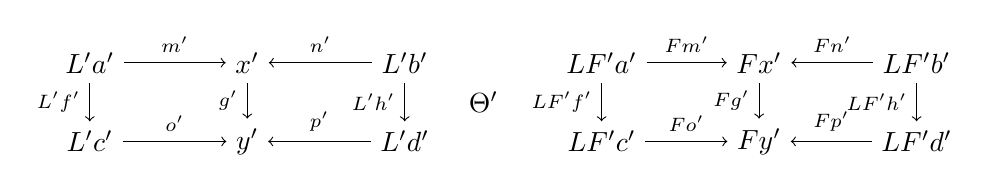
\begin{tikzpicture}
    \begin{scope}
      \node (1) at (-2,1) {\( L'a' \)};
      \node (2) at (0,1) {\( x' \)};
      \node (3) at (2,1) {\( L'b' \)};
      \node (4) at (-2,0) {\( L'c' \)};
      \node (5) at (0,0) {\( y' \)};
      \node (6) at (2,0) {\( L'd' \)};
      \draw [->] (1) to node [above] {\scriptsize{\( m' \)}} (2);
      \draw [->] (3) to node [above] {\scriptsize{\( n' \)}} (2);
      \draw [->] (4) to node [above] {\scriptsize{\( o' \)}} (5);
      \draw [->] (6) to node [above] {\scriptsize{\( p' \)}} (5);
      \draw [->] (1) to node [left] {\scriptsize{\( L'f' \)}} (4);
      \draw [->] (2) to node [left] {\scriptsize{\( g' \)}} (5);
      \draw [->] (3) to node [left] {\scriptsize{\( L'h' \)}} (6);
    \end{scope}
    %
    \begin{scope}[shift={(3,0)}]
      \node (1) at (0,0.5) { $ \xmapsto{ \Theta' } $ };
    \end{scope}
    % 
    \begin{scope}[shift={(6.5,0)}]
        \node (1) at (-2,1) {\( LF'a' \)};
        \node (2) at (0,1) {\( Fx' \)};
        \node (3) at (2,1) {\( LF'b' \)};
        \node (4) at (-2,0) {\( LF'c' \)};
        \node (5) at (0,0) {\( Fy' \)};
        \node (6) at (2,0) {\( LF'd' \)};
        \draw [->] (1) to node [above] {\scriptsize{\( Fm' \)}} (2);
        \draw [->] (3) to node [above] {\scriptsize{\( Fn' \)}} (2);
        \draw [->] (4) to node [above] {\scriptsize{\( Fo' \)}} (5);
        \draw [->] (6) to node [above] {\scriptsize{\( Fp' \)}} (5);
        \draw [->] (1) to node [left] {\scriptsize{\( LF'f' \)}} (4);
        \draw [->] (2) to node [left] {\scriptsize{\( Fg' \)}} (5);
        \draw [->] (3) to node [left] {\scriptsize{\( LF'h' \)}} (6);  
    \end{scope}
  \end{tikzpicture}\end{center}
\end{theorem}
\begin{proof}
  In light of Theorem \ref{thm:strcsp-istopos}, it suffices
  to show that $ \Theta \dashv \Theta' $ gives a geometric
  morphism.

  Denote the structured cospans
  $$[ m,n ] \colon La \to x \gets Lb$$ in $ _L\StrCsp $
  by $ \ell $ and $$[m',n'] \colon L'a' \to x' \gets L'b'$$ in
  $ _{ L' }\StrCsp $ by $ \ell' $. Denote the unit and
  counit for $F \dashv G$ by $ \eta $, $ \varepsilon $ and
  for $ F' \dashv G' $ by $ \eta' $, $ \varepsilon' $.  The
  assignments
  
  \begin{align*}
    \left( (f,g,h)\from\ell\to\Theta'\ell' \right)
      & \mapsto
        \left( (\epsilon'\circ F'f,
        \epsilon\circ Fg,
        \epsilon'\circ F'h )
        \from\Theta\ell\to\ell'\right) \\
    \left( (f',g',h')\from\Theta\ell\to\ell'\right)
      & \mapsto
        \left( (G'f'\circ\eta',Gg'\circ\eta,G'h'\circ\eta')
        \from\ell\to\Theta'\ell'\right) 
  \end{align*}
  
  give a bijection
  $ \hom (\Theta\ell,\ell') \simeq \hom (\ell,\Theta'\ell'
  )$. Moreover, it is natural in $\ell$ and $\ell'$. This
  rests on the natural maps $\eta$, $\epsilon$, $\eta'$, and
  $\epsilon'$. The left adjoint $\Theta'$ preserves finite
  limits because they are taken pointwise and $ L $, $ F $,
  and $ F' $ all preserve finite limits.
\end{proof}

With this theorem, we have highlighted categories of the
form $ _L\StrCsp $ where $ L $ runs through finite limit
preserving left adjoints. These \df{structured cospan
  categories} fit into a 2-category $ \SStrCsp $. A 1-arrow
from $ _L\StrCsp \to _{L'}\StrCsp $ is a pair of finitely
continuous and cocontinuous functors $ F \from \X \to \X' $
and $ G \from \A \to \A' $ fitting into the commuting
diagram
\begin{center}
  \begin{tikzpicture}
    \node (X) at (0,2) {$ \X $};
    \node (A) at (0,0) {$ \A $};
    \node (X') at (2,2) {$ \X' $};
    \node (A') at (2,0) {$ \A' $};
    \draw [cd] 
    (A) edge[bend left=20] node[left]{$ L $} (X)
    (X) edge[bend left=20] node[right]{$ R $} (A)
    (A') edge[bend left=20] node[left]{$ L' $} (X')
    (X') edge[bend left=20] node[right]{$ R' $} (A')
    (X) edge[] node[above]{$ F $} (X')
    (A) edge[] node[below]{$ G $} (A');
  \end{tikzpicture}
\end{center}
. A 2-arrow from $
(F,G) \To (F',G') $ is a pair of natural transformations $
\alpha \from F \To F' $ and $ \beta \from G \to G'$. 

%% =========================================
\section{Rewriting structured cospans}
\label{sec:RewritingStrCsp}
%% =========================================

\Daniel{Generalize gadducci/heckle's theorem.  Place it into
  the ACT context.}

\Daniel{require that L have monic counit from the start}


In Definition \ref{def:grammar}, we defined a category
$ \Gram $ where an object is a topos paired with a set of
rewrite rules and an arrow $ (\T , P) \to ( \T' , P' )$ is a
rule-preserving functor $ \T \to \T' $.  Our interest now
lies in the subcategory of structured cospan grammars
$ \StrCspGram $ that is full on the grammars where $ \T $ is
a structured cospan category and $ P $ is a set of structured
cospan rewrite rules.   

It is on this category $ \StrCspGram $ that we define the
\emph{language functor}
$ \Lang \from \StrCspGram \to \DblCat $ which encodes the
rewrite relation to each grammar. The ``language functor''
is an appropriate name as it provides \emph{(i)} the terms
formed by connecting together open systems (instead of
concatenating units of syntax in linguistics) and \emph{(ii)}
the rules governing how to interchange open systems (instead
of parts of speech). To help visualize this, we sketch a
simple example.

\begin{example}
  Starting with the discrete graph adjunction
  \[
    \adjunction{\RGraph}{L}{R}{\Set}
  \]
  for which $ _L \StrCsp $ is the category of open graphs,
  consider a grammar defined by the single rule
  \input{assets/singleRuleGrammar1.tex} The language
  associated to this grammar consists of all open
  graphs. The rewrite relation $ \deriv{g}{h} $ means that
  we obtained $ h $ by removing loops from $ g $. We
  illustrate this with the following square in the double
  category $ \Lang ( _L \StrCsp , P )
  $. \begin{center}\begin{tikzpicture}[scale=0.75]
    \begin{scope}[shift={(0,0)}] % up left
      \node (a) at (0,-1) {$ \bullet $};
      \node (b) at (0,1) {$ \bullet $};
      %
      \draw [rounded corners] (-2,-2) rectangle (2,2);
      \node (00r) at (2.1,0) {};
      \node (00b) at (0,-2.1) {};  
    \end{scope}
    %
    \begin{scope}[shift={(5,0)}] % up mid
      \node (a) at (-1,-1) {$ \bullet $};
      \node (b) at (-1,1) {$ \bullet $};
      \node (c) at (0,0) {$ \bullet $};
      \node (d) at (1,0) {$ \bullet $};
      %
      \draw [graph]
        (b) edge[loop above, looseness=15] (b)
        (c) edge[loop above, looseness=15] (c)
        (a) edge[] (c)
        (b) edge[] (c)
        (c) edge[] (d); 
      %  
      \draw [rounded corners] (-2,-2) rectangle (2,2);
      \node (01l) at (-2.1,0) {};
      \node (01r) at (2.1,0)  {};
      \node (01b) at (0,-2.1) {};  
    \end{scope}
    %
    \begin{scope}[shift={(10,0)}] % up right
      \node () at (0,0) {$ \bullet $};
      %
      \draw [rounded corners] (-2,-2) rectangle (2,2);
      \node (02l) at (-2.1,0) {};
      \node (02b) at (0,-2.1) {};
    \end{scope}
    % ~~~~~~~~~~~~~~~~~~~~~~~~~~~~~
    \begin{scope}[shift={(0,-5)}] % mid left
      \node () at (0,-1) {$ \bullet $};
      \node () at (0,1) {$ \bullet $};
      %
      \draw [rounded corners] (-2,-2) rectangle (2,2);
      \node (10t) at (0,2.1)   {};
      \node (10r) at (2.1,0) {};
      \node (10b) at (0,-2.1)  {};  
    \end{scope}
    %
    \begin{scope}[shift={(5,-5)}] % mid mid
      \node (a) at (-1,-1) {$ \bullet $};
      \node (b) at (-1,1) {$ \bullet $};
      \node (d) at (1,0) {$ \bullet $};
      %
      \draw [rounded corners] (-2,-2) rectangle (2,2);
      \node (11l) at (-2.1,0) {};
      \node (11r) at (2.1,0)  {};
      \node (11t) at (0,2.1)  {};
      \node (11b) at (0,-2.1) {};  
    \end{scope}
    %
    \begin{scope}[shift={(10,-5)}] % mid right
      \node () at (0,0) {$ \bullet $};
      %
      \draw [rounded corners] (-2,-2) rectangle (2,2);
      \node (12l) at (-2.1,0) {};
      \node (12t) at (0,2.1)    {};  
      \node (12b) at (0,-2.1)   {};
    \end{scope}
    % ~~~~~~~~~~~~~~~~~~~~~
    \begin{scope}[shift={(0,-10)}] % down left
      \node () at (0,-1) {$ \bullet $};
      \node () at (0,1) {$ \bullet $};
      %
      \draw [rounded corners] (-2,-2) rectangle (2,2);
      \node (20t) at (0,2.1)   {};
      \node (20r) at (2.1,0) {};
      \node (20b) at (0,-2.1)  {};  
    \end{scope}
    %
    \begin{scope}[shift={(5,-10)}] % down mid
      \node (a) at (-1,-1) {$ \bullet $};
      \node (b) at (-1,1) {$ \bullet $};
      \node (c) at (0,0) {$ \bullet $};
      \node (d) at (1,0) {$ \bullet $};
      %
      \draw [graph]
        (a) edge[] (c)
        (b) edge[] (c)
        (c) edge[] (d); 
      %
      \draw [rounded corners] (-2,-2) rectangle (2,2);
      \node (21l) at (-2.1,0) {};
      \node (21r) at (2.1,0)  {};
      \node (21t) at (0,2.1)  {};
      \node (21b) at (0,-2.1) {};  
    \end{scope}
    %
    \begin{scope}[shift={(10,-10)}] % down right
      \node () at (0,0) {$ \bullet $};
      %
      \draw [rounded corners] (-2,-2) rectangle (2,2);
      \node (22l) at (-2.1,0) {};
      \node (22r) at (2.1,0)  {};
      \node (22t) at (0,2.1)  {};
      \node (22b) at (0,-2.1) {};
    \end{scope}
    % ~~~~~~~~~~~~~~~~~~~
    \path[cd]
      (00r) edge (01l)
      (02l) edge (01r)
      (10r) edge (11l)
      (12l) edge (11r)
      (20r) edge (21l)
      (22l) edge (21r)
      (10t) edge[] (00b)
      (10b) edge[] (20t)
      (11t) edge[] (01b)
      (11b) edge[] (21t)
      (12t) edge[] (02b)
      (12b) edge[] (22t); ;
    \end{tikzpicture}\end{center}
\end{example}

We construct $ \Lang $ in two steps. First, we apply a
functor $ D \from \StrCspGram \to \StrCspGram $ that sends a
grammar $ ( _L \StrCsp , P ) $ to all of the rewrite rules
derived from $ P $. Second, we apply a functor
$ S \from \StrCspGram \to \DblCat $. that generates a double
category on the squares obtained from the rewrite rules of a
grammar $ ( _L \StrCsp , P ) $. In this way, we get the
language of a grammar as a double category where the squares
are the rewrite rules.  The next lemma defines $ D $ and
extracts some of its properties.

\begin{lemma}
  There is an idempotent functor
  $ D \from \StrCspGram \to \StrCspGram $ defined as
  follows. On objects define $ D ( _{L}\StrCsp , P ) $ to be
  the grammar $ ( _{L} \StrCsp , P_D) $, where $ P_D $
  consists of all rules $ \spn{g}{h}{d} $ witnessing the
  relation $ \dderiv{g}{h} $ with respect to
  $ ( _{L}\StrCsp , P ) $. On arrows, define
  $ DF \from D( _{L}\StrCsp , P ) \to D( _{L'}\StrCsp , Q )
  $ to be $ F $.  Moreover, the identity on $ \StrCspGram $
  is a subfunctor of $ D $.
\end{lemma}

\begin{proof}
  That $ D ( _{L}\StrCsp , P ) $ actually gives a grammar
  follows from the fact that pushouts respect monics in a
  topos \cite[Lem.~12]{LackSobo_Adhesive}.
  
  To show that $ \D $ is idempotent, we show that for any
  grammar $ ( _{L}\StrCsp , P ) $, we have
  $ D ( _{L}\StrCsp , P ) = DD ( _{L}\StrCsp , P ) $.  Rules
  in $ DD ( _{L}\StrCsp , P ) $ appear in the bottom row of a
  double pushout diagram whose top row is a rule in
  $ D ( _{L}\StrCsp , P ) $, which in turn is the bottom row
  of a double pushout diagram whose top row is in
  $ ( _{L}\StrCsp , P ) $. Thus, a rule in
  $ DD ( _{L}\StrCsp , P ) $ is the bottom row of a double
  pushout diagram whose top row is in
  $ ( _{L}\StrCsp , P ) $. See Figure \ref{fig:idempotentD}.

  \begin{figure}[h]
    \centering
    \fbox{
    \begin{minipage}{\linewidth}
    \vspace{2em}    
    \[
    \begin{tikzpicture}
      \node (1) at (0,4) {$ g $};
      \node (2) at (2,4) {$ d $};
      \node (3) at (4,4) {$ h $};
      \node (4) at (0,2) {$ g' $};
      \node (5) at (2,2) {$ d' $};
      \node (6) at (4,2) {$ h' $};
      \node (7) at (0,0) {$ g'' $};
      \node (8) at (2,0) {$ d'' $};
      \node (9) at (4,0) {$ h'' $};
      \draw [cd] (2) to node [] {\scriptsize{$  $}} (1);
      \draw [cd] (2) to node [] {\scriptsize{$  $}} (3);
      \draw [cd] (5) to node [] {\scriptsize{$  $}} (4);
      \draw [cd] (5) to node [] {\scriptsize{$  $}} (6);
      \draw [cd] (8) to node [] {\scriptsize{$  $}} (7);
      \draw [cd] (8) to node [] {\scriptsize{$  $}} (9);
      \draw [cd] (1) to node [] {\scriptsize{$  $}} (4);
      \draw [cd] (2) to node [] {\scriptsize{$  $}} (5);
      \draw [cd] (3) to node [] {\scriptsize{$  $}} (6);
      \draw [cd] (4) to node [] {\scriptsize{$  $}} (7);
      \draw [cd] (5) to node [] {\scriptsize{$  $}} (8);
      \draw [cd] (6) to node [] {\scriptsize{$  $}} (9);
      %
      \draw (0.3,0.4) -- (0.4,0.4) -- (0.4,0.3);
      \draw (3.7,0.4) -- (3.6,0.4) -- (3.6,0.3);   
      \draw (0.3,2.4) -- (0.4,2.4) -- (0.4,2.3);
      \draw (3.7,2.4) -- (3.6,2.4) -- (3.6,2.3);   
    \end{tikzpicture}
    \]
    \caption{Stacked double pushout diagrams}
    \label{fig:idempotentD}
  \end{minipage}
}
\end{figure}

  The identity is a subfunctor of $ D $ because the identity
  on any rule $ \spn{\ell}{k}{r} $ in
  $ ( _{L}\StrCsp , P ) $ induces $ \dderiv{\ell}{r} $.
  Hence there is a monomorphism
  \[
    ( _L \StrCsp , P ) \to
    D ( _L \StrCsp , P )
  \]
  induced from the identity functor on $ _L\StrCsp $.
\end{proof}

Plainly stated, $ D $ sends a grammar to a new grammar
consisting of all derived rules.  That $ D $ is idempotent
means that a rule derived from $ P $ can be derived
directly, hence multiple applications of $ D $ are
unnecessary.  That the identity is a subfunctor of $ D $
means that set of the derived rules $ P_D $ contains rules
in $ P $.

The next stage in defining $ \Lang $ is to define
$ S \from \StrCspGram \to \DblCat $. On objects, let
$ S ( _L \StrCsp , P ) $ be the sub-double category of
$ _L \SSStrCsp $ generated by the rules in $ P $ considered
as squares.  On arrows, $ S $ sends
\[
  F \from ( _{L}\StrCsp , P ) \to ( _{L'} \StrCsp , P' )
\]
to the double functor defined that extends the mapping
between the generators of $ S ( _{L}\StrCsp , P ) $ and
$ S ( _{L'}\StrCsp , P' ) $.  This preserves composition because
$ F $ preserves pullbacks and pushouts. 

\begin{definition}(Language of a grammar)
  The \df{language functor} is defined to be
  $ \Lang \coloneqq SD $. 
\end{definition}

To witness the rewriting relation on a closed system as a
square in a double category, we require this next lemma
that formalizes the analogy between rewriting the disjoint
union of systems and tensoring squares.

\begin{lemma} \label{thm:rewrite-rel-is-additive}
  If $ \deriv{x}{y} $ and $ \deriv{x'}{y'} $, then
  $ \deriv{x+x'}{y+y'} $
\end{lemma}

\begin{proof}
  If the derivation $ \deriv{x}{y} $ comes from a string of
  double pushout diagrams
  \begin{center}\begin{tikzpicture}[scale=0.75]
    \node (1t) at (0,2) {$ \ell_1 $};
    \node (2t) at (2,2) {$ k_1 $};
    \node (3t) at (4,2) {$ r_1 $};
    \node (4t) at (6,2) {$ \ell_2 $};
    \node (5t) at (8,2) {$ k_2 $};
    \node (6t) at (10,2) {$ r_2 $};
%    \node (7t) at (11,2) {$ \ell_n $};
    \node (8t) at (11,2) {$ k_n $};
    \node (9t) at (13,2) {$ r_n $};
    \node (1b) at (0,0) {$ x $};
    \node (2b) at (2,0) {$ d_1 $};
    \node (3b) at (5,0) {$ w_1 $};
    \node (4b) at (8,0) {$ d_2 $};
    \node (5b) at (10,0) {$ w_2 $};
%    \node (6b) at (11,0) {$ w_{n-1} $};
    \node (7b) at (11,0) {$ d_n $};
    \node (8b) at (13,0) {$ y $};
    \draw [cd] (2t) to node [] {\scriptsize{$  $}} (1t);
    \draw [cd] (2t) to node [] {\scriptsize{$  $}} (3t);
    \draw [cd] (5t) to node [] {\scriptsize{$  $}} (4t);
    \draw [cd] (5t) to node [] {\scriptsize{$  $}} (6t);
%    \draw [cd] (8t) to node [] {\scriptsize{$  $}} (7t);
    \draw [cd] (8t) to node [] {\scriptsize{$  $}} (9t);
    \draw [cd] (2b) to node [] {\scriptsize{$  $}} (1b);
    \draw [cd] (2b) to node [] {\scriptsize{$  $}} (3b);
    \draw [cd] (4b) to node [] {\scriptsize{$  $}} (3b);
    \draw [cd] (4b) to node [] {\scriptsize{$  $}} (5b);
%    \draw [cd] (7b) to node [] {\scriptsize{$  $}} (6b);
    \draw [cd] (7b) to node [] {\scriptsize{$  $}} (8b);
    \draw [cd] (1t) to node [] {\scriptsize{$  $}} (1b);
    \draw [cd] (2t) to node [] {\scriptsize{$  $}} (2b);
    \draw [cd] (3t) to node [] {\scriptsize{$  $}} (3b);
    \draw [cd] (4t) to node [] {\scriptsize{$  $}} (3b);
    \draw [cd] (5t) to node [] {\scriptsize{$  $}} (4b);
    \draw [cd] (6t) to node [] {\scriptsize{$  $}} (5b);
 %   \draw [cd] (7t) to node [] {\scriptsize{$  $}} (6b);
    \draw [cd] (8t) to node [] {\scriptsize{$  $}} (7b);
    \draw [cd] (9t) to node [] {\scriptsize{$  $}} (8b);
    \node () at (10.5,1) {$ \dotsm $};
    % 
    \draw (0.3,0.4) -- (0.4,0.4) -- (0.4,0.3);
    \draw (4.7,0.4) -- (4.6,0.4) -- (4.6,0.3);
    \draw (5.3,0.4) -- (5.4,0.4) -- (5.4,0.3);
    \draw (9.7,0.4) -- (9.6,0.4) -- (9.6,0.3);
 %   \draw (11.3,0.4) -- (11.4,0.4) -- (11.4,0.3);
    \draw (12.7,0.4) -- (12.6,0.4) -- (12.6,0.3);
  \end{tikzpicture}\end{center}
%  and the derivation
  $ \deriv{x'}{y'} $ comes from a string of double pushout
  diagrams % 
\begin{center} \begin{tikzpicture}[scale=0.8]
  \node (1t) at (0,2) {$ \ell'_1 $};
  \node (2t) at (2,2) {$ k'_1 $};
  \node (3t) at (4,2) {$ r'_1 $};
  \node (4t) at (6,2) {$ \ell'_2 $};
  \node (5t) at (8,2) {$ k'_2 $};
  \node (6t) at (10,2) {$ r'_2 $};
  \node (7t) at (11,2) {$ \ell'_m $};
  \node (8t) at (13,2) {$ k'_m $};
  \node (9t) at (15,2) {$ r'_m $};
  \node (1b) at (0,0) {$ x' $};
  \node (2b) at (2,0) {$ d'_1 $};
  \node (3b) at (5,0) {$ w'_1 $};
  \node (4b) at (8,0) {$ d'_2 $};
  \node (5b) at (10,0) {$ w'_2 $};
  \node (6b) at (11,0) {$ w'_{m-1} $};
  \node (7b) at (13,0) {$ d'_m $};
  \node (8b) at (15,0) {$ y' $};
  \draw [cd] (2t) to node [] {\scriptsize{$  $}} (1t);
  \draw [cd] (2t) to node [] {\scriptsize{$  $}} (3t);
  \draw [cd] (5t) to node [] {\scriptsize{$  $}} (4t);
  \draw [cd] (5t) to node [] {\scriptsize{$  $}} (6t);
  \draw [cd] (8t) to node [] {\scriptsize{$  $}} (7t);
  \draw [cd] (8t) to node [] {\scriptsize{$  $}} (9t);
  \draw [cd] (2b) to node [] {\scriptsize{$  $}} (1b);
  \draw [cd] (2b) to node [] {\scriptsize{$  $}} (3b);
  \draw [cd] (4b) to node [] {\scriptsize{$  $}} (3b);
  \draw [cd] (4b) to node [] {\scriptsize{$  $}} (5b);
  \draw [cd] (7b) to node [] {\scriptsize{$  $}} (6b);
  \draw [cd] (7b) to node [] {\scriptsize{$  $}} (8b);
  \draw [cd] (1t) to node [] {\scriptsize{$  $}} (1b);
  \draw [cd] (2t) to node [] {\scriptsize{$  $}} (2b);
  \draw [cd] (3t) to node [] {\scriptsize{$  $}} (3b);
  \draw [cd] (4t) to node [] {\scriptsize{$  $}} (3b);
  \draw [cd] (5t) to node [] {\scriptsize{$  $}} (4b);
  \draw [cd] (6t) to node [] {\scriptsize{$  $}} (5b);
  \draw [cd] (7t) to node [] {\scriptsize{$  $}} (6b);
  \draw [cd] (8t) to node [] {\scriptsize{$  $}} (7b);
  \draw [cd] (9t) to node [] {\scriptsize{$  $}} (8b);
  \node () at (10.5,1) {$ \dotsm $};
  % 
  \draw (0.3,0.4) -- (0.4,0.4) -- (0.4,0.3);
  \draw (4.7,0.4) -- (4.6,0.4) -- (4.6,0.3);
  \draw (5.3,0.4) -- (5.4,0.4) -- (5.4,0.3);
  \draw (9.7,0.4) -- (9.6,0.4) -- (9.6,0.3);
  \draw (11.3,0.4) -- (11.4,0.4) -- (11.4,0.3);
  \draw (14.7,0.4) -- (14.6,0.4) -- (14.6,0.3);
\end{tikzpicture} \end{center} realize
  $ \deriv{x+x'}{y+y'} $ by
  \begin{center} \begin{tikzpicture}[scale=0.8]
  \node (1t) at (0,2) {$ \ell_1 $};
  \node (2t) at (2,2) {$ k_1 $};
  \node (3t) at (4,2) {$ r1 $};
  \node () at (5,1) {$ \cdots $};
  \node (4t) at (6,2) {$ r_n $};
  \node (5t) at (8,2) {$ \ell'_1 $};
  \node (6t) at (10,2) {$ k'_1 $};
  \node (7t) at (12,2) {$ r'_1 $};
  \node () at (13,1) {$ \cdots $};
  \node (8t) at (14,2) {$ k'_m $};
  \node (9t) at (16,2) {$ r'_m $};
  % 
  \node (1b) at (0,0) {$ x+x' $};
  \node (2b) at (2,0) {$ d_1+x' $};
  \node (3b) at (4,0) {$ w_1+x' $};
  \node (5b) at (7,0) {$ y+x' $};
  \node (6b) at (10,0) {$ y+d'_1 $};
  \node (7b) at (12,0) {$ y+w'_1 $};
  \node (8b) at (14,0) {$ y+d'_m $};
  \node (9b) at (16,0) {$ y+y' $};
  % 
  \draw [cd]
    (2t) edge[] (1t)
    (2t) edge[] (3t)
    (6t) edge[] (5t)
    (6t) edge[] (7t)
    (8t) edge[] (9t) 
    (2b) edge[] (1b)
    (2b) edge[] (3b)
    (6b) edge[] (5b)
    (6b) edge[] (7b)
    (8b) edge[] (9b) 
    (1t) edge[] (1b)
    (2t) edge[] (2b)
    (3t) edge[] (3b)
    (4t) edge[] (5b)
    (5t) edge[] (5b)
    (6t) edge[] (6b)
    (7t) edge[] (7b)
    (8t) edge[] (8b)
    (9t) edge[] (9b);      
  \end{tikzpicture} \end{center}
\end{proof}

%% =====================================================
\section{A double category of structured cospan rewrites}
\label{sec:DblCat}
%% =====================================================

\Daniel{Cover what a grammar is and organize them into a double
category a la FineRewrite. Uncertain to include: interchange
law, symmetric monoidal structure. Just point to thesis?
Dno't call things FineRewrite, just Rewrite.}

Because $ _L\StrCsp $, the category of structured cospans
and their morphisms, is a topos, we are ensured that
rewriting structured cospans have a nice theory of rewriting
a l\'{a} adhesive categories \cite{LackSobo_Adhesive}.
The goal of this section is to define a double category whose squares
are rewrites of structured cospans.  The rough idea is
that this double category, denoted $ _L\RRRewrite $, has
``interface'' types for objects, structured cospans for
horizontal arrows, isomorphisms of interface objects for
vertical arrows, and rewrite rules of structured
cospans for squares. We prove in Proposition
\ref{thm:fine-rewrite-double-cat} that $ _L\RRRewrite $
actually is a double category. The first step to proving
this is to ensure the rewrite rules are suitable squares for
our double category, we define them as follows.

\begin{definition}[Rewrite]
  A \df{rewrite rule of structured cospans} is an
  isomorphism class of spans of structured cospans of the
  form \[
  \begin{tikzpicture}[
    baseline=(current bounding box.center),
    scale=0.75]
    \node (a) at (0,4) {$ La $};
    \node (b) at (2,4) {$ x $};
    \node (c) at (4,4) {$ Lb $};
    \node (x) at (0,2) {$ Lc $};
    \node (y) at (2,2) {$ y $};
    \node (z) at (4,2) {$ Ld $};
    \node (d) at (0,0) {$ Le $};
    \node (e) at (2,0) {$ z$};
    \node (f) at (4,0) {$ Lf $};
    %    
    \draw [>->] (y) to (b);
    \draw [>->] (y) to (e);
    \draw[cd]
    (a) edge[] (b)
    (x) edge[] (y)
    (d) edge[] (e)
    (c) edge[] (b)
    (z) edge[] (y)
    (f) edge[] (e)
    (x) edge[] node[left]{$ \iso $}  (a)
    (z) edge[] node[right]{$ \iso $} (c)
    (x) edge[] node[left]{$ \iso $}  (d)
    (z) edge[] node[right]{$ \iso $} (f) ;
  \end{tikzpicture}
\]
 The marked arrows are
  monic.
\end{definition}

Working with isomorphism classes is a technical point.  The
squares of a double category are subject to two composition
operations. Below, we define horizontal composition using
pushout, as is standard with cospan categories, and vertical
composition uses pullback, as is standard in span
categories.  But pushouts and pullbacks are defined only up
to isomorphism and there are no higher order arrows
traversing the squares in a double category. Therefore, we
must work with isomorphism classes of structured cospan
rewrite rules.

The \df{horizontal composition} of rewrite rules is given by
\input{assets/horComposition1.tex} We interpret this as
taking composable open systems, each undergoing a rewrite,
and combining them into a single open system undergoing a
single rewrite.

The \df{vertical composition} of rewrite rules is given by
\input{assets/vertComposition.tex} We interpret this as an open
system undergoing a two-step rewrite.  

Here, we must make two technical points. The first is that
horizontal and vertical composition are defined on
representatives of isomorphism classes and one can show that
operation is well-defined. The second is that we require the
monic arrows to be preserved, which we show in Proposition
\ref{thm:comp-preserve-monic} below. To prove this
proposition, we requires the following lemma.

\begin{lemma}
  \label{thm:quotient-map-monic-pushout}
  The diagram   \begin{equation} \label{eq:qmmp-1}
    \begin{tikzpicture}
      \node (x) at  (0,2) {$ x $};
      \node (y) at  (2,2) {$ y $};
      \node (z) at  (4,2) {$ z $};
      \node (x') at (0,0) {$ x' $};
      \node (y') at (2,0) {$ y' $};
      \node (z') at (4,0) {$ z' $};
      %
      \draw [cd]  (y) edge (x);
      \draw [cd]  (y) edge (z);
      \draw [cd]  (y') edge (x');
      \draw [cd]  (y') edge (z');
      \draw [>->] (x) edge (x');
      \draw [cd]  (y) edge node[left]{$ \iso $} (y');
      \draw [>->] (z) edge (z');
    \end{tikzpicture}
  \end{equation}
  %
  induces a pushout
  \input{assets/quotientMapMonicPushout2.tex} such that the
  canonical arrows $ \gamma $ and $ \gamma' $ are monic.
\end{lemma}

\begin{proof}
  The universal property of coproducts implies
  that $ \gamma $ factors through $ x' + z $ as in
  the diagram %
  \[
    \begin{tikzpicture}
      \node (x) at (0,4) {$ x $};
      \node (x') at (0,2) {$ x' $};
      \node (x+z) at (2,4) {$ x+z $};
      \node (x'+z) at (2,2) {$ x'+z $};
      \node (x'+z') at (2,0) {$ x'+z' $};
      \node (z) at (4,2) {$ z $};
      \node (z') at (4,0) {$ z' $};
      %
      \draw [>->] (x) to node[above]{$ \iota_x $}  (x+z);
      \draw [>->] (x') to node[below]{$ \iota_{x'} $} (x'+z);
      \draw [>->] (z) to node[above]{$ \iota_z  $} (x'+z);
      \draw [>->] (z') to node[below]{$ \iota_{z'} $} (x'+z');
      \draw [>->] (x) to (x');
      \draw [cd] (x+z) to (x'+z);
      \draw [cd] (x'+z) to (x'+z');
      \draw [>->] (z) to (z');
    \end{tikzpicture}
  \]
  %
   
  It is straightforward to check that both squares are
  pushouts. By Lemma \ref{lem:adhesive-properties}, it
  follows that $ \gamma $ is monic.

  Diagram \ref{eq:qmmp-2} commutes because of the universal
  property of coproducts.  To see that it is a pushout,
  arrange a cocone
  \input{assets/quotientMapMonicPushout4.tex}
  
  Denote by $ \iota_x $ any map that includes $ x $.  Then
  $ \psi' \iota_{x'} $, $ \psi' \iota_{z'} $, and $ c $ form
  a cocone under the span $ x' \gets y' \to z' $ from the
  bottom face of Diagram \ref{eq:qmmp-1}. This induces the
  canonical map $ \psi'' \from x'+_{y'} z' \to c $. It
  follows that
  $ \psi' \iota_{x'} = \psi'' \rho' \iota_{x'} $ and
  $ \psi' \iota_{z'} = \psi'' \rho' \iota_{z'} $. Therefore
  $ \psi' = \psi'' \rho' $ by the universal property of
  coproducts.

  Furthermore, $ \psi \rho \iota_z $,
  $ \psi \rho \iota_z $, and $ c $ form a cocone
  under the span $ x \gets y \to z $ on the top
  face of Diagram \ref{eq:qmmp-1}. then
  $ \psi \rho \iota_x = \psi' \gamma \iota_x =
  \psi'' \rho' \gamma \iota_x = \psi'' \psi' \rho
  \iota_x $ and
  $ \psi \rho \iota_z = \psi' \gamma \iota_z =
  \psi'' \rho' \gamma \iota_z = \psi'' \gamma'
  \rho \iota_z $ meaning that both $ \psi $ and
  $ \psi'' \psi' $ satisfy the canonical map
  $ x+_yz \to d $. Hence $ \psi = \psi'' \psi' $.

  The universality of $ \psi'' $ with respect to
  Diagram \ref{eq:qmmp-3} follows from the
  universality of $ \gamma'' $ with respect to
  $ x'+_{y'}z' $.
\end{proof}

\begin{proposition} \label{thm:comp-preserve-monic}
  Horizontal and vertical composition preserve rewrite rules
  of structured cospans.
\end{proposition}

\begin{proof}
  For the horizontal composition of
  rewrites \input{assets/compPreserveMonic1.tex}, the arrows 
  $ w +_{Le} x \to u+_{Lb} v $ and
  $ w +_{Le} x \to y +_{Lh} z $ are monic. This is seen by applying
  Lemma \ref{thm:quotient-map-monic-pushout} to the diagrams
  \input{assets/compPreserveMonic2.tex}
  
  The result for vertical composition holds because pullback
  preserves monomorphisms.

  % \input{assets/compPreserveMonic3.tex} is the diagram eq
  % for vert comp.
\end{proof}

With horizontal and vertical composition in hand, we
construct the double category $ _L\RRRewrite $.
Actually, we delay discussing the interchange law until
Section \ref{sec:interchange-law} because it is difficult
enough to warrant its own section.

\begin{proposition}
\label{thm:rewrite-double-cat}
  Let
  \[
    \adjunction{\X}{L}{R}{\A}
  \]
  be a adjunction with $ L $ preserving pullbacks.  There is
  a double category $ _L\RRRewrite $ whose objects are the
  $ \A $-objects, horizontal arrows of type $ a \to b $ are
  structured cospans $ La \to x \gets Lb $, vertical arrows
  of type $ a \to b $ are isomorphism classes of spans
  $ a \gets c \to b $ in $ \A $ with invertible arrows, and
  squares are rewrites of structured cospans
  \[
    \begin{tikzpicture}
    \node (La)   at (0,4) {$ La $};
    \node (x)    at (2,4) {$ x $};
    \node (Lb)   at (4,4) {$ La' $};
    \node (La')  at (0,2) {$ Lb $};
    \node (x')   at (2,2) {$ y $};
    \node (Lb')  at (4,2) {$ Lb' $};
    \node (La'') at (0,0) {$ Lc $};
    \node (x'')  at (2,0) {$ z $};
    \node (Lb'') at (4,0) {$ Lc' $};
    \draw [cd] (La)   to (x);
    \draw [cd] (Lb)   to (x);
    \draw [cd] (La')  to (x');
    \draw [cd] (Lb')  to (x');
    \draw [cd] (La'') to (x'');
    \draw [cd] (Lb'') to (x'');
    \draw [cd] (La')  to
      node [left] {$ \iso $} (La);
    \draw [>->] (x') to (x);
    \draw [cd] (Lb') to
      node [right] {$ \iso $} (Lb);
    \draw [cd] (La') to
      node [left] {$ \iso $} (La'');
    \draw [>->] (x') to (x'');
    \draw [cd] (Lb') to
      node [right] {$ \iso $} (Lb'');
    \end{tikzpicture}
  \]
\end{proposition}

\begin{proof}
  This proof requires we check the axioms of a double
  category. For simplicity, we denote $_L\RRRewrite$ by
  $\RRR $ in this proof.

  The object category $\RRR_0$ is given by objects of $\A$
  and isomorphism classes of spans in $\A$ such that each
  leg is an isomorphism.  The arrow category $\RRR_1$ has as
  objects the structured cospans
  \[
    La \to x \gets La'
  \]
  and as morphisms the fine rewrites of structured cospans.
	
  The functor $U \from \RRR_0 \to \RRR_1$ acts on objects by
  mapping $a$ to the identity cospan on $La$ and on
  morphisms by mapping $La \gets Lb \to Lc$, whose legs are
  isomorphisms, to the square
  \input{assets/rewriteDoubleCat2.tex}
  
  The functor $S \from \RRR_1 \to \RRR_0$ acts on objects by
  sending $La \to x \gets La'$ to $a$ and on morphisms by
  sending a square \input{assets/rewriteDoubleCat3.tex}
  
  to the span $ La \gets Lb \to Lc $. The functor $T$ is
  defined similarly sends an object \[ La \to x \gets La' \]
  of $ \RRR_1 $ to $ a' $ a square
  \[
    \begin{tikzpicture}
      \node (A) at (0,4) {$La$};
      \node (A') at (0,2) {$Lb$};
      \node (A'') at (0,0) {$Lc$};
      \node (B) at (2,4) {$x$};
      \node (B') at (2,2) {$y$};
      \node (B'') at (2,0) {$z$};
      \node (C) at (4,4) {$La'$};
      \node (C') at (4,2) {$Lb'$};
      \node (C'') at (4,0) {$Lc'$};
      % 
      \draw[cd]
      % horizontal arrows
      (A) edge node{} (B)
      (A') edge node{} (B')
      (A'') edge node{} (B'')
      (C) edge node{} (B)
      (C') edge node{} (B')
      (C'') edge node{} (B'')
      % vertical arrows
      (A') edge node{} (A)
      (A') edge node{} (A'')
      (B') edge node{} (B)
      (B') edge node{} (B'')
      (C') edge node{} (C)
      (C') edge node{} (C'');
    \end{tikzpicture}
  \] to the span
  $ La' \gets Lb' \to Lc' $.
  
  The horizontal composition functor
  \[
    \odot \from \RRR_1 \times_{\RRR_0} \RRR_1 \to
    \RRR_1
  \]
  acts on objects by composing cospans with pushouts in the
  usual way.  It acts on morphisms by
  \[
    \raisebox{-0.5\height}{
      \begin{tikzpicture}
        \node (A) at (0,4) {$La$};
        \node (A') at (0,2) {$Lb$};
        \node (A'') at (0,0) {$Lc$};
        \node (B) at (2,4) {$v$};
        \node (B') at (2,2) {$w$};
        \node (B'') at (2,0) {$x$};
        \node (C) at (4,4) {$La'$};
        \node (C') at (4,2) {$Lb'$};
        \node (C'') at (4,0) {$Lc'$};
        \node (D) at (6,4) {$v'$};
        \node (D') at (6,2) {$w'$};
        \node (D'') at (6,0) {$x'$};
        \node (E) at (8,4) {$La''$};
        \node (E') at (8,2) {$Lb''$};
        \node (E'') at (8,0) {$Lc''$};
        % 
        \draw[cd]
        % horizontal arrows
        (A) edge node[above]{} (B)
        (A') edge node[above]{} (B')
        (A'') edge node[above]{} (B'')
        (C) edge node[above]{} (B)
        (C') edge node[above]{} (B')
        (C'') edge node[above]{} (B'')
        (C) edge node[above]{} (D)
        (C') edge node[above]{} (D')
        (C'') edge node[above]{} (D'')
        (E) edge node[above]{} (D)
        (E') edge node[above]{} (D')
        (E'') edge node[above]{} (D'')
        % vertical arrows
        (A') edge node[left]{} (A)
        (A') edge node[left]{} (A'')
        (B') edge node[left]{} (B)
        (B') edge node[left]{} (B'')
        (C') edge node[left]{} (C)
        (C') edge node[left]{} (C'')	
        (D') edge node[left]{} (D)
        (D') edge node[left]{} (D'')
        (E') edge node[left]{} (E)
        (E') edge node[left]{} (E'');
      \end{tikzpicture}
    }
    \quad
    \xmapsto{\odot}
    \quad
    \raisebox{-0.5\height}{
      \begin{tikzpicture}
        \node (A) at (0,4) {$La$};
        \node (A') at (0,2) {$Lb$};
        \node (A'') at (0,0) {$Lc$};
        \node (B) at (2,4) {$v +_{La'} v'$};
        \node (B') at (2,2) {$w +_{Lb'} w'$};
        \node (B'') at (2,0) {$x +_{Lc'} x'$};
        \node (C) at (4,4) {$La''$};
        \node (C') at (4,2) {$Lb''$};
        \node (C'') at (4,0) {$Lc''$};
        % 
        \draw[cd]
        % horizontal arrows
        (A) edge node[above]{} (B)
        (A') edge node[above]{} (B')
        (A'') edge node[above]{} (B'')
        (C) edge node[above]{} (B)
        (C') edge node[above]{} (B')
        (C'') edge node[above]{} (B'')
        % vertical arrows
        (A') edge node[left]{} (A)
        (A') edge node[left]{} (A'')
        (B') edge node[left]{} (B)
        (B') edge node[left]{} (B'')
        (C') edge node[left]{} (C)
        (C') edge node[left]{} (C'');	
      \end{tikzpicture}
    }
  \]

  The interchange law holds
  \cite[Lem.~4.3]{CicCour_SpCspTopos}, therefore $\odot$ is
  a functor. It is straightforward to check that the
  required equations are satisfied.  The associator and
  unitors are given by natural isomorphisms that arise from
  universal properties.
\end{proof}

And now, our double category of rewrites is defined.


%% =====================================================
\section{Expressiveness of grammars}
\label{sec:gen-result-graph-rewriting}
%% =====================================================

For a rewrite rule $ \ell \gets k \to r $, there is no
constraint on the value of $ k $. Even though we interpret
it as being the suboject of $ \ell $ and $ r $ that remains
fixed through the application of the rule, it can actually
be any object of the topos in which we are working.  Such
freedom is difficult to work with, so we devise a more
restrained alternative. That is, we ask that $ k $ be
\emph{discrete}. In this section, we make the term
`discrete' precise and show that the rewriting relation of a
grammar $ (\T,P) $ is the same as the discretized variant of
$ (\T,P) $. This result generalizes a characterization of
discrete graph grammars given by Ehrig,
et.~al. \cite[Prop.~3.3]{Ehrig_GraphGram}.

Experts in topos theory may recognize `discreteness' from
the flat modality on a local topos. However, we avoid the
lengthy detour required to discuss what a `flat modality'
and a `local topos' actually are because it would not add to
our story (curious readers can find this information elsewhere
\cite[Ch.~C3.6]{Johnstone_Sketches}). The cost of avoiding
this detour is one comonad.

The definition of the `discrete comonad' is straightforward
enough, but its purpose may seem alien at first. After the
definition, we explain its role in rewriting structured
cospans.

\begin{definition}[Discrete comonad]
  \label{def:discrete-comonad}
  A comonad on a topos is called \df{discrete} if its counit
  is monic. We use $ \flat $ to denote a discrete comonad.
\end{definition}

Secretly, we have been working with a discrete comonad all
along. The adjunction $$\adjunction{\RGraph}{L}{R}{\Set}$$
induces the comonad $ LR $ on $ \RGraph $.  Applying $ LR $ to
a graph $ x $ returns the edgeless graph underlying $
x $, hence the term `discrete'. For example \begin{center}\begin{tikzpicture}
    \begin{scope}
      \node (a) at (0,2) {$ \bullet $};
      \node (b) at (2,1) {$ \bullet $};
      \node (c) at (0,0) {$ \bullet $};
      %
      \draw [graph] 
        (a) edge[] (b)
        (a) edge[] (c)
        (b) edge[] (c);
      %
      \draw [rounded corners] (-1,-1) rectangle (3,3);
    \end{scope}
    %
    \begin{scope}[shift={(6,0)}]
      \node (a) at (0,2) {$ \bullet $};
      \node (b) at (2,1) {$ \bullet $};
      \node (c) at (0,0) {$ \bullet $};
      %
      \draw [rounded corners] (-1,-1) rectangle (3,3);
    \end{scope}
    %
    \draw [|->] (3.5,1) to node[above]{$ LR $} (4.5,1);
\end{tikzpicture}\end{center} 

The counit $ \epsilon_x \from LRx \to x $ of the comonad
$ LR $ includes the underlying edgeless graph $ LRx $ into
the original graph $ x $. For example, \input{assets/includeEdgelessGraphEx.tex}

Abstractly, this inclusion is why we ask for the counit to
be monic. The property we capture with a discrete comonad
comes from the systems interpretation of the
adjunctions $$\adjunction{\X}{L}{R}{\A}$$ between
topoi. That is, $ R $ takes a system $ x $, identifies the
largest sub-system that can serve as an interface and turns
that sub-system into an interface type $ Rx $. Then $ L $
takes that interface type and turns it back into a system
$ LRx $. This process effectively strips away every part of
a system leaving only those parts that can connect to the
outside world. That means $ LRx $ is a part of $ x $ or, in
the parlance of category theory, $ LRx $ is a subobject of
$ x $.  Hence, we ask for a monic counit.

How do we plan to use discrete comonads?  We use them to
control the form of our grammars. In particular, we can \emph{discretize} any rewrite
rule $$\ell \gets k \to r$$ by replacing $ k $ with
$ \flat k $.  

\begin{definition}[Discrete grammar]
  Given a grammar $ ( \X , P ) $, define $ P_\flat $ as the set
  consisting of a rule
  \[ \ell \gets k \gets \flat k \to k \to r \]
  for each rule $ \ell \gets k \to r $ in $ P $. We call $
  ( X , P_\flat ) $ the \df{discrete grammar} underlying $
  ( \X, P ) $.
\end{definition}

Theorem \ref{thm:production-same-rewrite-relation-as-discrete} gives
a sufficient condition that allows us to swap $ ( \X,P ) $
for $ ( \X,P_\flat ) $ without consequence. The proof of this theorem borrows from lattice theory, so let us digress from rewriting to fill in the requisit background.

\begin{definition}[Lattice]
  A lattice is a poset $ ( S, \leq ) $ equipped with all
  finite joins $ \bigvee $ and all finite meets
  $ \bigwedge $. It follows that there is a minimal 0 element
  and maximal element 1, realized as the empty meet and join,
  respectively.
\end{definition}

Joins and meets are also known as suprema and infima. We are
using the definition of a lattice common in the category
theory literature. This leaves out objects that some
mathematicians might consider lattices. Below we give one
counter-example and several examples of lattices, the last
one being the most relevant.

\begin{example}[Integer Lattice]
  The integers with the usual ordering $ \leq $ do not form
  a lattice because there is no minimal or maximal element.
\end{example}

\begin{example}[Lattice of power sets]
  For any set $ S $, its powerset $ \mathcal{P}S $ is a
  poset via subset inclusion. The powerset becomes a lattice
  by taking join to be union $ a \vee b \bydef a \cup b $,
  and meet to be intersection $ a \wedge b \bydef a \cap b
  $. In general, union and intersection are defined over
  arbitrary sets, thus realizing arbitrary joins
  $ \bigvee a_\alpha $ and arbitrary meets
  $ \bigwedge a_\alpha $. 
\end{example}

Those few examples provide intuition about lattices, but the
next example is the most important lattice for us. It is the
mechanism by which the power set is generalized into topos
theory. It is called the subobject lattice.

\begin{example}[Subobject lattice]
  Let $ \T $ be a topos and $ t $ be an object. There is a
  lattice $ \Sub (t) $ called the subobject lattice of
  $ t $.  The elements of $ \Sub (t) $, called
  subobjects, are isomorphism classes of monomorphisms
  into $ t $. Here, two monomorphisms $ f,g $ into $ t $ are
  isomorphic if there is a commuting diagram \begin{center}
\begin{tikzpicture}
      \node (a) at (-1,2) {$ a $};
      \node (b) at (1,2) {$ b $};
      \node (t) at (0,0) {$ t $};
      \draw [cd] 
      (a) edge[] node[left]{$ f $} (t)
      (b) edge[] node[right]{$ g $} (t)
      (a) edge[] node[above]{$ \iso $} (b); 
    \end{tikzpicture}
  \end{center}
  
  The order on $ \Sub (t) $ is given by $ f \leq g $ if
  $ f $ factors through $ g $, meaning there is an arrow
  $ h \from a \to b $ such that $ f = gh $. Note that $ h $
  is necessarily monic. The meet operation in $ \Sub (t) $
  is given by pullback \input{assets/meetPullback.tex} and
  join is given by pushout over the meet
  \begin{center}\begin{tikzpicture}
      \node (ab) at (0,2) {$ a \vee b $};
      \node (a)  at (0,0) {$ a $};
      \node (b)  at (2,2) {$ b $};
      \node (t)  at (2,0) {$ a \wedge b $};
      \node (tt) at (4,-2) {$ t $};
      %
      \draw [cd] 
      (ab) edge[]           (a)
      (ab) edge[]           (b)
      (a)  edge[]           (t)
      (b)  edge[]           (t)
      (a)  edge[bend right] (tt)
      (b)  edge[bend left]  (tt);
      \draw [->,dashed] (t) edge (tt) ;
      %
      \draw (1.7,0.4) -- (1.6,0.4) -- (1.6,0.3);
  \end{tikzpicture}\end{center}
\end{example}

Subobject lattices provide a way to compare the expressivity of a grammar to its underlying discrete grammar.
To do
this, we require a subobject lattice with arbitrary meets.  The
powerset lattice mentioned above has this property, but
when does a subobject lattice have this property?  Here are
several sufficient conditions, starting with a well-known
result from order theory.

\begin{proposition} \label{thm:lattice-alljoins-allmeets}
  Any lattice that has all joins also has all meets.
\end{proposition}

\begin{proof}
  Consider a subset $ S $ of a lattice. Define the meet of $
  S $ to be the join of the set of all lower bounds of $ S $.
\end{proof}

\begin{proposition} \label{thm:subob-arbitrary-meets}
  Fix an object $t$ of a topos $ \T $.  The subobject
  lattice $ \Sub (t) $ has arbitrary meets when the over-category 
	$ T \downarrow t $ has all products.
\end{proposition}

\begin{proof}
  Because $ T \downarrow t $ is a topos, it has
  equalizers. Thus giving it all products ensures the
  existence of all limits, hence meets. 
\end{proof}

\begin{corollary}
  Fix an object $t$ of a topos $ \T $.  The subobject
  lattice $ \Sub (t) $ has arbitrary meets when the over
  category $ T \downarrow t $ has all coproducts.
\end{corollary}

\begin{proof}
  Combine Propositions \ref{thm:lattice-alljoins-allmeets}
  and \ref{thm:subob-arbitrary-meets}.
\end{proof}

The case where $\T$ is a presheave category is especially pertinent to us because, often, a system can be encoded as a presheaf. Labelled graphs offer a large cache of examples.

At last, we combine the discrete comonad, the discrete
grammar, and the complete subobject lattice into a result on
the expressiveness on discrete grammars.

\begin{theorem}
  \label{thm:production-same-rewrite-relation-as-discrete}  
  Let $ \T $ be a topos and $ \flat \from \T \to \T $ be a
  discrete comonad.  Let $ ( \T , P ) $ be a grammar such
  that for every rule $ \ell \gets k \to r $ in $ P $, the
  subobject lattice $ \Sub (k) $ has all meets. Then the
  rewriting relation for $ ( \T , P ) $ equals the
  rewriting relation for the underlying discrete grammar
  $ ( \T,P_\flat ) $.
\end{theorem}

\begin{proof}
  Suppose that $ ( \T,P ) $ induces $ \dderiv{g}{h} $. That
  means there exists a rule $ \spn{\ell}{k}{r} $ in $ P $
  and a derivation \input{assets/expressivityProof1.tex}
  
  we can achieve that same derivation using rules in
  $ P_\flat $. This requires we build a pushout complement
  $ w $ of the diagram \begin{center}\begin{tikzpicture}
      \node (k) at (0,2) {$ k $};
      \node (bk) at (2,2) {$ \flat k $};
      \node (d) at (0,0) {$ d $};
      %
      \draw [cd]
        (bk) edge[] node[above]{$ \epsilon $} (k)
        (k) edge[] (d); 
  \end{tikzpicture}\end{center}

  Define
  \[ w \coloneqq \bigwedge \{ z \colon z \vee k = d \} \vee
    \flat k,\] This comes with inclusions $ \flat k \to w $
  and $ w \to d $. This $ w $ exists because $ \Sub (k) $
  has all meets.  Note that $ w \vee k = d $ and
  $ w \wedge k = \flat k $ which means that
  \[\begin{tikzpicture}[scale=0.75]
      \node (k) at (0,2) {$ k $};
      \node (bk) at (2,2) {$ \flat k $};
      \node (d) at (0,0) {$ d $};
      \node (w) at (2,0) {$ w $};
      %
      \draw [cd] 
      (bk) edge[] (k)
      (bk) edge[] (w)
      (k) edge[] (d)
      (w) edge[] (d);
      %
      \draw (0.3,0.4) -- (0.4,0.4) -- (0.4,0.3);
  \end{tikzpicture}\] is a pushout. It
  follows that there is a derivation
  %
  \begin{equation} \label{eq:prod-rewrite-2}
  \begin{tikzpicture}
    \node (01) at (0,2) {$ \ell $};
    \node (11) at (2,2) {$ k $};
    \node (21) at (4,2) {$ \flat k $};
    \node (31) at (6,2) {$ k $};
    \node (41) at (8,2) {$ r $};
    \node (00) at (0,0) {$ g $};
    \node (10) at (2,0) {$ d $};
    \node (20) at (4,0) {$ w $};
    \node (30) at (6,0) {$ d $};
    \node (40) at (8,0) {$ h $};
    %
    \draw [cd] (11) to node [] {\scriptsize{$  $}} (01);
    \draw [cd] (21) to node [] {\scriptsize{$  $}} (11);
    \draw [cd] (21) to node [] {\scriptsize{$  $}} (31);
    \draw [cd] (31) to node [] {\scriptsize{$  $}} (41);
    \draw [cd] (10) to node [] {\scriptsize{$  $}} (00);
    \draw [cd] (20) to node [] {\scriptsize{$  $}} (10);
    \draw [cd] (20) to node [] {\scriptsize{$  $}} (30);
    \draw [cd] (30) to node [] {\scriptsize{$  $}} (40);
    \draw [cd] (01) to node [] {\scriptsize{$  $}} (00);
    \draw [cd] (11) to node [] {\scriptsize{$  $}} (10);
    \draw [cd] (21) to node [] {\scriptsize{$  $}} (20);
    \draw [cd] (31) to node [] {\scriptsize{$  $}} (30);
    \draw [cd] (41) to node [] {\scriptsize{$  $}} (40);
    %
    \draw (0.3,0.4) -- (0.4,0.4) -- (0.4,0.3);
    \draw (2.3,0.4) -- (2.4,0.4) -- (2.4,0.3);
    \draw (5.7,0.4) -- (5.6,0.4) -- (5.6,0.3);
    \draw (7.7,0.4) -- (7.6,0.4) -- (7.6,0.3);
  \end{tikzpicture}\end{equation} with respect to
  $ P_\flat $ because, the top row is a rule in $ P_\flat $.
  Therefore, $ \dderiv{g}{h} $ via $ P $ in Diagram
  \eqref{eq:prod-rewrite-1} implies that $ \deriv{g}{h} $
  via $ P_\flat $ as shown in Diagram
  \eqref{eq:prod-rewrite-2}.

  For the other direction, suppose $ \dderiv{g}{h} $ via
  $ P_\flat $, giving a derivation
  \begin{equation}
  \label{eq:prod-rewrite-3}
  \begin{tikzpicture}
    \node (1t) at (0,2) {$ \ell $};
    \node (2t) at (2,2) {$ \flat k $};
    \node (3t) at (4,2) {$ r $};
    \node (1b) at (0,0) {$ g $};
    \node (2b) at (2,0) {$ d $};
    \node (3b) at (4,0) {$ h $};
    \draw [cd]
      (2t) edge                          (1t)
      (2t) edge                          (3t)
      (2b) edge node[below]{$ \psi $}    (1b)
      (2b) edge                          (3b)
      (1t) edge node[left]{$ m $}        (1b)
      (2t) edge node[left]{$ \theta $}   (2b)
      (3t) edge node[right]{$ m' $}      (3b);
      %
      \draw (0.3,0.4) -- (0.4,0.4) -- (0.4,0.3);
      \draw (3.7,0.4) -- (3.6,0.4) -- (3.6,0.3);
  \end{tikzpicture}
\end{equation}

  By construction of $ P_\flat $, the rule
  $ \spn{\ell}{\flat k}{r} $ in $ P_\flat $ was induced from
  a rule $$\ell \xgets{\tau} k \to r$$ in $ P $, meaning
  that the map $ \flat k \to \ell $ factors through
  $ \tau $. Next, define $ d' $ to be the pushout of the
  diagram \begin{center}\begin{tikzpicture}
  \node (flatk) at (0,2) {$ \flat k $};
  \node (k)     at (2,2) {$ k $};
  \node (d)     at (0,0) {$ d $};
  \node (d')    at (2,0) {$ d' $};
  % 
  \draw [cd] 
   (flatk) edge[] node[above]{$ \epsilon $}       (k)
   (flatk) edge[] node[left]{$ \theta $}          (d)
   (d)     edge[] node[below]{$ \hat{\epsilon} $} (d')
   (k)     edge[] node[right]{$ \hat{\theta} $}   (d');
  % 
  \draw (1.7,0.4) -- (1.6,0.4) -- (1.6,0.3);
\end{tikzpicture}\end{center}

  By invoking the universal property of this pushout with
  the maps
  \[
    \psi \from d \to g \quad \text{and} \quad m \tau \from k
    \to \ell \to g,
  \]
  we get a canonical map $ d' \to g $ that we can fit into a
  commuting diagram \input{assets/expressivityProof7.tex}
  whose back faces are pushouts. Using a standard diagram
  chasing argument, we can show that the front face is also
  a pushout.  Similarly, the square
  \begin{center}\begin{tikzpicture}
  \node (k) at (0,2) {$ k $};
  \node (r) at (2,2) {$ r $};
  \node (d') at (0,0) {$ d' $};
  \node (h) at (2,0) {$ h $};
  % 
  \draw [cd] 
    (k) edge[] (r)
    (k) edge[] (d')
    (d') edge[] (h)
    (r) edge[] (h);
  % 
  \draw (1.7,0.4) -- (1.6,0.4) -- (1.6,0.3);
\end{tikzpicture}\end{center} is a pushout.  Sticking
  these two pushouts together
  \begin{center}\begin{tikzpicture}[scale=0.75]
  \node (1t) at (0,2) {$ \ell $};
  \node (2t) at (2,2) {$ k $};
  \node (3t) at (4,2) {$ r $};
  \node (1b) at (0,0) {$ g $};
  \node (2b) at (2,0) {$ d' $};
  \node (3b) at (4,0) {$ h $};
  \draw [cd]
    (2t) edge                     (1t)
    (2t) edge                     (3t)
    (2b) edge                     (1b)
    (2b) edge                     (3b)
    (1t) edge node[left]{$ m $}   (1b)
    (2t) edge node[left]{$ \hat{\theta} $}   (2b)
    (3t) edge node[right]{$ m' $} (3b);
  \draw (0.3,0.4) -- (0.4,0.4) -- (0.4,0.3);
  \draw (3.7,0.4) -- (3.6,0.4) -- (3.6,0.3);
\end{tikzpicture}\end{center} shows that
  $ \dderiv{g}{h} $ arises from $ P $.

  Because the relation $ \dderiv{}{} $ is the same for $ P $
  and $ P_\flat $, it follows that $ \deriv{}{} $ is also
  the same as claimed.
\end{proof}




%% =======================================
%% =======================================

\section{Characterizing the rewrite relation for closed
  systems}
\label{sec:charRewrRelat}

Here, we apply the theory of rewriting structured cospans to
classifying the rewrite relation for closed systems. We start
by formalizing closed systems as structured cospans with an
empty interface $ L0 \to x \gets L0 $. In other words,
closed systems are particular horizontal 1-arrows in the
double category $ _L \RRRewrite $.  To decompose a closed
system $$L0 \to x \gets L0$$ is to write an arrow as a
composite of arrows
\[
  L0 \to x_1 \gets La_1 \to x_2 \gets La_2 \to
  \dotsm \gets La_{n-1} \to x_n \gets L0
\]
We use such decompositions to prove our main result which
states that two structured cospans
\[
  L0 \to x \gets L0
  \quad \text{and} \quad
  L0 \to x' \gets L0
\]
are equivalent precisely when there is a square between
them.  We interpret this result in three ways.

\begin{enumerate}
\item It shows that the rewriting relation for a closed system
  is functorial and is characterized using squares in a double
  category.
\item A closed system decomposes into open systems and
  simplifying each open system simplifies the composite
  closed system.  
\item Open systems provide a local perspective on closed
  systems via this decomposition.
\end{enumerate}

To decompose closed systems into open systems, we need a
topos of closed systems $ \X $ equipped with a grammar
$ ( \X , P ) $. The closed systems need interfaces, meaning
we need to introduce an adjunction
\[
  \adjunction{\X}{L}{R}{\A}
\]
where $ L $ preserves pullbacks and has a monic counit. At
this point, the material from the previous section
returns. This adjunction gives a discrete comonad $ \flat
\bydef LR $ from which we form the discrete
grammar $ ( \X, P_\flat ) $. Now define the structured cospan
grammar $ ( _L \StrCsp , \hat{P_\flat} ) $ where $
\hat{P_\flat} $ contains the rule \begin{equation} \label{eq:decomposition-square}
  \begin{tikzpicture}
    \node (1) at (0,4) {$ L 0 $};
    \node (2) at (2,4) {$ \ell $};
    \node (3) at (4,4) {$ LRk $};
    \node (4) at (0,2) {$ L 0 $};
    \node (5) at (2,2) {$ LRk $};
    \node (6) at (4,2) {$ LRk $};
    \node (7) at (0,0) {$ L 0 $};
    \node (8) at (2,0) {$ r $};
    \node (9) at (4,0) {$ LRk $};
    \draw [cd] (1) to (2);
    \draw [cd] (3) to (2);
    \draw [cd] (4) to (5);
    \draw [cd] (6) to (5);
    \draw [cd] (7) to (8);
    \draw [cd] (9) to (8);
    \draw [cd] (4) to (1);
    \draw [cd] (4) to (7);
    \draw [cd] (5) to (2);
    \draw [cd] (5) to (8);
    \draw [cd] (6) to (3);
    \draw [cd] (6) to (9);
  \end{tikzpicture}
\end{equation}
% 
for each rule $ \spn{\ell}{LRk}{r} $ of $ P_{\flat} $. We
use $ ( _L \StrCsp , \hat{P_\flat} ) $ to prove our main
theorem.

Before stating the theorem, we note that this theorem
generalizes work by Gadducci and Heckel
\cite{Gadd_IndGraphTrans} whose domain of
inquiry was graph rewriting. The arc of our
proof follows theirs.


\begin{theorem} \label{thm:inductive-rewriting}
  Fix an adjunction $ (L \dashv R) \from \X \lrto \A $ with
  monic counit. Let $ ( \X , P ) $ be a grammar such that
  for every $ \X $-object $ x $ in the apex of a production
  of $ P $, the lattice $ \Sub (x) $ has all meets. Given
  $ g $, $ h \in \X $, then $ \deriv{g}{h} $ in the
  rewriting relation for a grammar $ ( \X , P ) $ if and
  only if there is a square
  %
  \begin{center} \begin{tikzpicture}[scale=0.75]
    \node (1t) at (0,4) {$ LR 0 $};
    \node (2t) at (2,4) {$ g $};
    \node (3t) at (4,4) {$ LR 0 $};
    \node (1m) at (0,2) {$ LR 0 $};
    \node (2m) at (2,2) {$ d $};
    \node (3m) at (4,2) {$ LR 0 $};
    \node (1b) at (0,0) {$ LR 0 $};
    \node (2b) at (2,0) {$ h $};
    \node (3b) at (4,0) {$ LR 0 $};
    % 
    \draw [cd] (1t) to node [] {\scriptsize{$  $}} (2t);
    \draw [cd] (3t) to node [] {\scriptsize{$  $}} (2t);
    \draw [cd] (1m) to node [] {\scriptsize{$  $}} (2m);
    \draw [cd] (3m) to node [] {\scriptsize{$  $}} (2m);
    \draw [cd] (1b) to node [] {\scriptsize{$  $}} (2b);
    \draw [cd] (3b) to node [] {\scriptsize{$  $}} (2b);
    \draw [cd] (1m) to node [] {\scriptsize{$  $}} (1t);
    \draw [cd] (1m) to node [] {\scriptsize{$  $}} (1b);
    \draw [cd] (2m) to node [] {\scriptsize{$  $}} (2t);
    \draw [cd] (2m) to node [] {\scriptsize{$  $}} (2b);
    \draw [cd] (3m) to node [] {\scriptsize{$  $}} (3t);
    \draw [cd] (3m) to node [] {\scriptsize{$  $}} (3b);
  \end{tikzpicture} \end{center}
  % 
  in the double category $ \Lang ( _{L}\StrCsp , \hat{P_\flat} ) $.
\end{theorem}

\begin{proof}
  We show sufficiency by inducting on the length of the
  derivation. If $ \deriv{g}{h} $ in a single step, meaning
  that there is a diagram
  %
  \begin{center}\begin{tikzpicture}
    \node (1t) at (0,2) {$ \ell $};
    \node (2t) at (2,2) {$ LRk $};
    \node (3t) at (4,2) {$ r $};
    \node (1b) at (0,0) {$ g $};
    \node (2b) at (2,0) {$ d $};
    \node (3b) at (4,0) {$ h $};
    \draw [cd] (2t) to (1t);
    \draw [cd] (2t) to (3t);
    \draw [cd] (2b) to (1b);
    \draw [cd] (2b) to (3b);
    \draw [cd] (1t) to (1b);
    \draw [cd] (2t) to (2b);
    \draw [cd] (3t) to (3b);
    %
    \draw (0.3,0.4) -- (0.4,0.4) -- (0.4,0.3);
    \draw (3.7,0.4) -- (3.6,0.4) -- (3.6,0.3);
  \end{tikzpicture} \end{center}
  % 
  then the desired square is the horizontal composition of
  %
  \begin{center} \begin{tikzpicture}
    \begin{scope}
      \node (1t) at (0,4) {$ L0 $};
      \node (2t) at (2,4) {$ \ell $};
      \node (3t) at (4,4) {$ LRk $};
      \node (4t) at (6,4) {$ d $};
      \node (5t) at (8,4) {$ L0 $};
      \node (1m) at (0,2) {$ L 0 $};
      \node (2m) at (2,2) {$ LRk $};
      \node (3m) at (4,2) {$ LRk $};
      \node (4m) at (6,2) {$ d $};
      \node (5m) at (8,2) {$ L 0 $};
      \node (1b) at (0,0) {$ L 0 $};
      \node (2b) at (2,0) {$ r $};
      \node (3b) at (4,0) {$ LRk $};
      \node (4b) at (6,0) {$ d $};
      \node (5b) at (8,0) {$ L 0 $};
      \draw [cd] (1t) to node [] {\scriptsize{$  $}} (2t);
      \draw [cd] (3t) to node [] {\scriptsize{$  $}} (2t);
      \draw [cd] (3t) to node [] {\scriptsize{$  $}} (4t);
      \draw [cd] (5t) to node [] {\scriptsize{$  $}} (4t);
      \draw [cd] (1m) to node [] {\scriptsize{$  $}} (2m);
      \draw [cd] (3m) to node [] {\scriptsize{$  $}} (2m);
      \draw [cd] (3m) to node [] {\scriptsize{$  $}} (4m);
      \draw [cd] (5m) to node [] {\scriptsize{$  $}} (4m);
      \draw [cd] (1b) to node [] {\scriptsize{$  $}} (2b);
      \draw [cd] (3b) to node [] {\scriptsize{$  $}} (2b);
      \draw [cd] (3b) to node [] {\scriptsize{$  $}} (4b);
      \draw [cd] (5b) to node [] {\scriptsize{$  $}} (4b);
      \draw [cd] (1m) to node [] {\scriptsize{$  $}} (1t);
      \draw [cd] (1m) to node [] {\scriptsize{$  $}} (1b);
      \draw [cd] (2m) to node [] {\scriptsize{$  $}} (2t);
      \draw [cd] (2m) to node [] {\scriptsize{$  $}} (2b);
      \draw [cd] (3m) to node [] {\scriptsize{$  $}} (3t);
      \draw [cd] (3m) to node [] {\scriptsize{$  $}} (3b);
      \draw [cd] (4m) to node [] {\scriptsize{$  $}} (4t);
      \draw [cd] (4m) to node [] {\scriptsize{$  $}} (4b);
      \draw [cd] (5m) to node [] {\scriptsize{$  $}} (5t);
      \draw [cd] (5m) to node [] {\scriptsize{$  $}} (5b);
    \end{scope}
  \end{tikzpicture}\end{center}
% 
  
  The left square is a generator and the right square is the
  identity on the horizontal arrow $ \csp{LRk}{d}{L0}
  $. The square for a derivation
  $ \dderiv{\deriv{g}{h}}{j} $ is the vertical composition
  of
  %
  \begin{center} \begin{tikzpicture}
    \node (1t) at (0,8) {$ L 0 $};
    \node (2t) at (2,8) {$ g $};
    \node (3t) at (4,8) {$ L 0 $};
    \node (1m) at (0,6) {$ L 0 $};
    \node (2m) at (2,6) {$ d $};
    \node (3m) at (4,6) {$ L 0 $};
    \node (1b) at (0,4) {$ L 0 $};
    \node (2b) at (2,4) {$ h $};
    \node (3b) at (4,4) {$ L 0 $};
    \node (1bb) at (0,2) {$ L 0 $};
    \node (2bb) at (2,2) {$ e $};
    \node (3bb) at (4,2) {$ L 0 $};
    \node (1bbb) at (0,0) {$ L 0 $};
    \node (2bbb) at (2,0) {$ j $};
    \node (3bbb) at (4,0) {$ L 0 $};
    \draw [cd] (1t) to node [] {\scriptsize{$  $}} (2t);
    \draw [cd] (3t) to node [] {\scriptsize{$  $}} (2t);
    \draw [cd] (1m) to node [] {\scriptsize{$  $}} (2m);
    \draw [cd] (3m) to node [] {\scriptsize{$  $}} (2m);
    \draw [cd] (1b) to node [] {\scriptsize{$  $}} (2b);
    \draw [cd] (3b) to node [] {\scriptsize{$  $}} (2b);
    \draw [cd] (1m) to node [] {\scriptsize{$  $}} (1t);
    \draw [cd] (1m) to node [] {\scriptsize{$  $}} (1b);
    \draw [cd] (2m) to node [] {\scriptsize{$  $}} (2t);
    \draw [cd] (2m) to node [] {\scriptsize{$  $}} (2b);
    \draw [cd] (3m) to node [] {\scriptsize{$  $}} (3t);
    \draw [cd] (3m) to node [] {\scriptsize{$  $}} (3b);
    \draw [cd] (1bb) to node [] {\scriptsize{$  $}} (2bb);
    \draw [cd] (3bb) to node [] {\scriptsize{$  $}} (2bb);
    \draw [cd] (1bbb) to node [] {\scriptsize{$  $}} (2bbb);
    \draw [cd] (3bbb) to node [] {\scriptsize{$  $}} (2bbb);
    \draw [cd] (1bb) to node [] {\scriptsize{$  $}} (1b);
    \draw [cd] (1bb) to node [] {\scriptsize{$  $}} (1bbb);
    \draw [cd] (2bb) to node [] {\scriptsize{$  $}} (2b);
    \draw [cd] (2bb) to node [] {\scriptsize{$  $}} (2bbb);
    \draw [cd] (3bb) to node [] {\scriptsize{$  $}} (3b);
    \draw [cd] (3bb) to node [] {\scriptsize{$  $}} (3bbb);
  \end{tikzpicture} \end{center}
  %
  
  The top square is from $ \deriv{g}{h} $ and the second
  from $ \dderiv{h}{j} $.

  Conversely, proceed by structural induction on the
  generating squares of
  $ \Lang ( _{L}\StrCsp , \hat{P_\flat} ) $.  It suffices to
  show that the rewrite relation is preserved by vertical
  and horizontal composition by generating squares.  Suppose
  we have a square
  %
  \begin{center}\begin{tikzpicture}
    \node (1t) at (0,4) {$ L 0 $};
    \node (2t) at (2,4) {$ w $};
    \node (3t) at (4,4) {$ L 0 $};
    \node (1m) at (0,2) {$ L 0 $};
    \node (2m) at (2,2) {$ x $};
    \node (3m) at (4,2) {$ L 0 $};
    \node (1b) at (0,0) {$ L 0 $};
    \node (2b) at (2,0) {$ y $};
    \node (3b) at (4,0) {$ L 0 $};
    \draw [cd] (2t) to node [] {\scriptsize{$  $}} (1t);
    \draw [cd] (2t) to node [] {\scriptsize{$  $}} (3t);
    \draw [cd] (2m) to node [] {\scriptsize{$  $}} (1m);
    \draw [cd] (2m) to node [] {\scriptsize{$  $}} (3m);
    \draw [cd] (2b) to node [] {\scriptsize{$  $}} (1b);
    \draw [cd] (2b) to node [] {\scriptsize{$  $}} (3b);
    \draw [cd] (1m) to node [] {\scriptsize{$  $}} (1t);
    \draw [cd] (2m) to node [] {\scriptsize{$  $}} (2t);
    \draw [cd] (3m) to node [] {\scriptsize{$  $}} (3t);
    \draw [cd] (1m) to node [] {\scriptsize{$  $}} (1b);
    \draw [cd] (2m) to node [] {\scriptsize{$  $}} (2b);
    \draw [cd] (3m) to node [] {\scriptsize{$  $}} (3b);
  \end{tikzpicture}\end{center}
  % 
  corresponding to a derivation $ \deriv{w}{y} $. Composing
  this vertically with a generating square, which must have
  form
  %
  \begin{center}\begin{tikzpicture}
    \node (1t) at (0,4) {$ L 0 $};
    \node (2t) at (2,4) {$ y $};
    \node (3t) at (4,4) {$ L 0 $};
    \node (1m) at (0,2) {$ L 0 $};
    \node (2m) at (2,2) {$ L 0 $};
    \node (3m) at (4,2) {$ L 0 $};
    \node (1b) at (0,0) {$ L 0 $};
    \node (2b) at (2,0) {$ z $};
    \node (3b) at (4,0) {$ L 0 $};
    \draw [cd] (2t) to node [] {\scriptsize{$  $}} (1t);
    \draw [cd] (2t) to node [] {\scriptsize{$  $}} (3t);
    \draw [cd] (2m) to node [] {\scriptsize{$  $}} (1m);
    \draw [cd] (2m) to node [] {\scriptsize{$  $}} (3m);
    \draw [cd] (2b) to node [] {\scriptsize{$  $}} (1b);
    \draw [cd] (2b) to node [] {\scriptsize{$  $}} (3b);
    \draw [cd] (1m) to node [] {\scriptsize{$  $}} (1t);
    \draw [cd] (2m) to node [] {\scriptsize{$  $}} (2t);
    \draw [cd] (3m) to node [] {\scriptsize{$  $}} (3t);
    \draw [cd] (1m) to node [] {\scriptsize{$  $}} (1b);
    \draw [cd] (2m) to node [] {\scriptsize{$  $}} (2b);
    \draw [cd] (3m) to node [] {\scriptsize{$  $}} (3b);
  \end{tikzpicture}\end{center}
  %
  corresponding to a production $ \spn{y}{L0}{z} $ gives
  %
  \begin{center}\begin{tikzpicture}
    \node (1t) at (0,4) {$ L 0 $};
    \node (2t) at (2,4) {$ w $};
    \node (3t) at (4,4) {$ L 0 $};
    \node (1m) at (0,2) {$ L 0 $};
    \node (2m) at (2,2) {$ L 0 $};
    \node (3m) at (4,2) {$ L 0 $};
    \node (1b) at (0,0) {$ L 0 $};
    \node (2b) at (2,0) {$ z $};
    \node (3b) at (4,0) {$ L 0 $};
    \draw [cd] (2t) to node [] {\scriptsize{$  $}} (1t);
    \draw [cd] (2t) to node [] {\scriptsize{$  $}} (3t);
    \draw [cd] (2m) to node [] {\scriptsize{$  $}} (1m);
    \draw [cd] (2m) to node [] {\scriptsize{$  $}} (3m);
    \draw [cd] (2b) to node [] {\scriptsize{$  $}} (1b);
    \draw [cd] (2b) to node [] {\scriptsize{$  $}} (3b);
    \draw [cd] (1m) to node [] {\scriptsize{$  $}} (1t);
    \draw [cd] (2m) to node [] {\scriptsize{$  $}} (2t);
    \draw [cd] (3m) to node [] {\scriptsize{$  $}} (3t);
    \draw [cd] (1m) to node [] {\scriptsize{$  $}} (1b);
    \draw [cd] (2m) to node [] {\scriptsize{$  $}} (2b);
    \draw [cd] (3m) to node [] {\scriptsize{$  $}} (3b);
  \end{tikzpicture}\end{center}
  %
  which corresponds to a derivation
  $ \dderiv{\deriv{w}{y}}{z} $.  Composing horizontally with
  a generating square
  %
  \begin{center}\begin{tikzpicture}
    \node (1t) at (0,4) {$ L 0 $};
    \node (2t) at (2,4) {$ \ell $};
    \node (3t) at (4,4) {$ L 0 $};
    \node (1m) at (0,2) {$ L 0 $};
    \node (2m) at (2,2) {$ LRk $};
    \node (3m) at (4,2) {$ L 0 $};
    \node (1b) at (0,0) {$ L 0 $};
    \node (2b) at (2,0) {$ r $};
    \node (3b) at (4,0) {$ L 0 $};
    \draw [cd] (2t) to node [] {\scriptsize{$  $}} (1t);
    \draw [cd] (2t) to node [] {\scriptsize{$  $}} (3t);
    \draw [cd] (2m) to node [] {\scriptsize{$  $}} (1m);
    \draw [cd] (2m) to node [] {\scriptsize{$  $}} (3m);
    \draw [cd] (2b) to node [] {\scriptsize{$  $}} (1b);
    \draw [cd] (2b) to node [] {\scriptsize{$  $}} (3b);
    \draw [cd] (1m) to node [] {\scriptsize{$  $}} (1t);
    \draw [cd] (2m) to node [] {\scriptsize{$  $}} (2t);
    \draw [cd] (3m) to node [] {\scriptsize{$  $}} (3t);
    \draw [cd] (1m) to node [] {\scriptsize{$  $}} (1b);
    \draw [cd] (2m) to node [] {\scriptsize{$  $}} (2b);
    \draw [cd] (3m) to node [] {\scriptsize{$  $}} (3b);
  \end{tikzpicture}\end{center}
  % 
  corresponding with a production $ \spn{\ell}{LRk}{r} $
  results in the square
  %
  \begin{center}\begin{tikzpicture}
    \node (1t) at (0,4) {$ L 0 $};
    \node (2t) at (2,4) {$ w + \ell $};
    \node (3t) at (4,4) {$ L 0 $};
    \node (1m) at (0,2) {$ L 0 $};
    \node (2m) at (2,2) {$ x + LRk $};
    \node (3m) at (4,2) {$ L 0 $};
    \node (1b) at (0,0) {$ L 0 $};
    \node (2b) at (2,0) {$ y + r $};
    \node (3b) at (4,0) {$ L 0 $};
    \draw [cd] (2t) to node [] {\scriptsize{$  $}} (1t);
    \draw [cd] (2t) to node [] {\scriptsize{$  $}} (3t);
    \draw [cd] (2m) to node [] {\scriptsize{$  $}} (1m);
    \draw [cd] (2m) to node [] {\scriptsize{$  $}} (3m);
    \draw [cd] (2b) to node [] {\scriptsize{$  $}} (1b);
    \draw [cd] (2b) to node [] {\scriptsize{$  $}} (3b);
    \draw [cd] (1m) to node [] {\scriptsize{$  $}} (1t);
    \draw [cd] (2m) to node [] {\scriptsize{$  $}} (2t);
    \draw [cd] (3m) to node [] {\scriptsize{$  $}} (3t);
    \draw [cd] (1m) to node [] {\scriptsize{$  $}} (1b);
    \draw [cd] (2m) to node [] {\scriptsize{$  $}} (2b);
    \draw [cd] (3m) to node [] {\scriptsize{$  $}} (3b);
  \end{tikzpicture}\end{center}
  %
  But $ \deriv{w+\ell}{y+r} $ as seen in Lemma
  \ref{thm:rewrite-rel-is-additive}. 
\end{proof}

With this result, we have completely described the rewrite
relation for a grammar $ ( \X , P ) $ with squares in
$ \Lang ( _{L}\StrCsp, \hat{P_\flat} ) $ framed by the
initial object of $ \X $.  These squares are rewrites of a
closed system in the sense that the interface is empty.  We
can instead begin with a closed system $ x $ in $ \X $ as
represented by a horizontal arrow $ \csp{L0}{x}{L0} $ in
$ \Lang ( _{L}\StrCsp , \hat{P_\flat} ) $ and decompose it
into a composite of sub-systems, that is a sequence of
composable horizontal arrows

\begin{center}\begin{tikzpicture}
  \node (L0) at (0,0) {$ L0 $};
  \node (x1) at (1,1) {$ x_1 $};
  \node (La1) at (2,0) {$ La_1 $};
  \node (x2) at (3,1) {$ x_2 $};
  \node (La2) at (4,0) {$ La_2 $};
  \node () at (5,0) {$ \dotsm $};
  \node (Lan1) at (6,0) {$ La_{n-1} $};
  \node (xn) at (7,1) {$ x_n $};
  \node (L0') at (8,0) {$ L0 $};
  % 
  \draw [cd] 
    (L0) edge[] (x1)
    (La1) edge[] (x1)
    (La1) edge[] (x2)
    (La2) edge[] (x2)
    (Lan1) edge[] (xn)
    (L0') edge[] (xn);
\end{tikzpicture}\end{center}

Rewriting can be performed on each of these sub-systems
%
\begin{center}\begin{tikzpicture}
\begin{scope}[shift={(0,6)}]
  \node (1) at (0,4) {$ L0 $};
  \node (2) at (2,4) {$ x_1 $};
  \node (3) at (4,4) {$ La_1 $};
  \node (4) at (0,2) {$ L0 $};
  \node (5) at (2,2) {$ x'_1 $};
  \node (6) at (4,2) {$ La'_1 $};
  \node (7) at (0,0) {$ L0 $};
  \node (8) at (2,0) {$ x''_1 $};
  \node (9) at (4,0) {$ La''_1 $};
  \draw [cd] (1) to (2);
  \draw [cd] (3) to (2);
  \draw [cd] (4) to (5);
  \draw [cd] (6) to (5);
  \draw [cd] (7) to (8);
  \draw [cd] (9) to (8);
  \draw [cd] (4) to node [left]
    {\scriptsize{$ \cong $}} (1);
  \draw [cd] (4) to node [left]
    {\scriptsize{$ \cong $}} (7);
  \draw [>->] (5) to (2);
  \draw [>->] (5) to (8);
  \draw [cd] (6) to node [right]
    {\scriptsize{$ \cong  $}} (3);
  \draw [cd] (6) to node [right]
    {\scriptsize{$ \cong $}} (9);
\end{scope}
% 
\begin{scope}[shift={(6,6)}]
  \node (1) at (0,4) {$ La_{n-1} $};
  \node (2) at (2,4) {$ x_n $};
  \node (3) at (4,4) {$ L0 $};
  \node (4) at (0,2) {$ La_{n-1} $};
  \node (5) at (2,2) {$ x'_n $};
  \node (6) at (4,2) {$ L0 $};
  \node (7) at (0,0) {$ La_{n-1} $};
  \node (8) at (2,0) {$ x''_n $};
  \node (9) at (4,0) {$ L0 $};
  \draw [cd] (1) to (2);
  \draw [cd] (3) to (2);
  \draw [cd] (4) to (5);
  \draw [cd] (6) to (5);
  \draw [cd] (7) to (8);
  \draw [cd] (9) to (8);
  \draw [cd] (4) to node [left]
    {\scriptsize{$ \cong $}} (1);
  \draw [cd] (4) to node [left]
    {\scriptsize{$ \cong $}} (7);
  \draw [>->] (5) to (2);
  \draw [>->] (5) to (8);
  \draw [cd] (6) to node [right]
    {\scriptsize{$ \cong  $}} (3);
  \draw [cd] (6) to node [right]
    {\scriptsize{$ \cong $}} (9);
\end{scope}
% 
\begin{scope}
  \node (1) at (0,4) {$ L0 $};
  \node (2) at (2,4) {$ y_1 $};
  \node (3) at (4,4) {$ La_1 $};
  \node (4) at (0,2) {$ L0 $};
  \node (5) at (2,2) {$ y'_1 $};
  \node (6) at (4,2) {$ La_1 $};
  \node (7) at (0,0) {$ L0 $};
  \node (8) at (2,0) {$ y''_1 $};
  \node (9) at (4,0) {$ La_1 $};
  \draw [cd] (1) to (2);
  \draw [cd] (3) to (2);
  \draw [cd] (4) to (5);
  \draw [cd] (6) to (5);
  \draw [cd] (7) to (8);
  \draw [cd] (9) to (8);
  \draw [cd] (4) to node[left]{$\cong$} (1);
  \draw [cd] (4) to node[left]{$\cong$} (7);
  \draw [>->] (5) to (2);
  \draw [>->] (5) to (8);
  \draw [cd] (6) to node[right]{$\cong$} (3);
  \draw [cd] (6) to node[right]{$\cong$} (9);
\end{scope}
% 
\begin{scope}[shift={(6,0)}]
  \node (1) at (0,4) {$ La_{n-1} $};
  \node (2) at (2,4) {$ y_n $};
  \node (3) at (4,4) {$ L0 $};
  \node (4) at (0,2) {$ La_{n-1} $};
  \node (5) at (2,2) {$ y'_n $};
  \node (6) at (4,2) {$ L0 $};
  \node (7) at (0,0) {$ La_{n-1} $};
  \node (8) at (2,0) {$y''_n $};
  \node (9) at (4,0) {$ L0 $};
  \draw [cd] (1) to (2);
  \draw [cd] (3) to (2);
  \draw [cd] (4) to (5);
  \draw [cd] (6) to (5);
  \draw [cd] (7) to (8);
  \draw [cd] (9) to (8);
  \draw [cd] (4) to node [left] {$\cong$} (1);
  \draw [cd] (4) to node [left] {$\cong$} (7);
  \draw [>->] (5) to (2);
  \draw [>->] (5) to (8);
  \draw [cd] (6) to node [right] {$\cong$} (3);
  \draw [cd] (6) to node [right] {$\cong$} (9);
\end{scope}
% 
\node () at (5,2) {$ \dotsm $};
\node () at (2,5) {$ \vdots $};
\node () at (5,8) {$ \dotsm $};
\node () at (8,5) {$ \vdots $};
\end{tikzpicture}\end{center}
%
The composite of these squares is a rewriting of the
original system.

\bibliographystyle{plain}
\bibliography{assets/biblio}



\end{document}

